
%% Copyright 2007-2024 Elsevier Ltd
%% 
%% This file is part of the 'Elsarticle Bundle'.
%% ---------------------------------------------
%% 
%% It may be distributed under the conditions of the LaTeX Project Public
%% License, either version 1.3 of this license or (at your option) any
%% later version.  The latest version of this license is in
%%    http://www.latex-project.org/lppl.txt
%% and version 1.3 or later is part of all distributions of LaTeX
%% version 1999/12/01 or later.
%% 
%% The list of all files belonging to the 'Elsarticle Bundle' is
%% given in the file `manifest.txt'.
%% 
%% Template article for Elsevier's document class `elsarticle'
%% with harvard style bibliographic references

% \documentclass[preprint,12pt,authoryear]{elsarticle}

%% Use the option review to obtain double line spacing
% \documentclass[authoryear,preprint,review,12pt]{elsarticle}

%% Use the options 1p,twocolumn; 3p; 3p,twocolumn; 5p; or 5p,twocolumn
%% for a journal layout:
% \documentclass[final,1p,times,authoryear]{elsarticle}
% \documentclass[final,1p,times,twocolumn,authoryear]{elsarticle}
\documentclass[final,3p,times,authoryear]{elsarticle}
% \documentclass[final,3p,times,twocolumn,authoryear]{elsarticle}
% \documentclass[final,5p,times,authoryear]{elsarticle}
% \documentclass[final,5p,times,twocolumn,authoryear]{elsarticle}

%% For including figures, graphicx.sty has been loaded in
%% elsarticle.cls. If you prefer to use the old commands
%% please give \usepackage{epsfig}

%% The amssymb package provides various useful mathematical symbols
\usepackage{amssymb}
%% The amsmath package provides various useful equation environments.
\usepackage{amsmath}
%% The amsthm package provides extended theorem environments
%% \usepackage{amsthm}
% for tables
\usepackage{makecell}

\usepackage{hyperref}
\usepackage{longtable}
%% The lineno packages adds line numbers. Start line numbering with
%% \begin{linenumbers}, end it with \end{linenumbers}. Or switch it on
%% for the whole article with \linenumbers.
%% \usepackage{lineno}

\journal{eclinicalmedicine}

\begin{document}

\begin{frontmatter}

%% Title, authors and addresses

%% use the tnoteref command within \title for footnotes;
%% use the tnotetext command for theassociated footnote;
%% use the fnref command within \author or \affiliation for footnotes;
%% use the fntext command for theassociated footnote;
%% use the corref command within \author for corresponding author footnotes;
%% use the cortext command for theassociated footnote;
%% use the ead command for the email address,
%% and the form \ead[url] for the home page:
%% \title{Title\tnoteref{label1}}
%% \tnotetext[label1]{}
%% \author{Name\corref{cor1}\fnref{label2}}
%% \ead{email address}
%% \ead[url]{home page}
%% \fntext[label2]{}
%% \cortext[cor1]{}
%% \affiliation{organization={},
%%            addressline={}, 
%%            city={},
%%            postcode={}, 
%%            state={},
%%            country={}}
%% \fntext[label3]{}

\title{A Machine Learning Model Built with Time-Dependent Lab Data to Predict Chronic Urticaria Duration and Provide Clinical Insights}

%% use optional labels to link authors explicitly to addresses:
%% \author[label1,label2]{}
%% \affiliation[label1]{organization={},
%%             addressline={},
%%             city={},
%%             postcode={},
%%             state={},
%%             country={}}
%%
%% \affiliation[label2]{organization={},
%%             addressline={},
%%             city={},
%%             postcode={},
%%             state={},
%%             country={}}

%% 作者和机构的对应关系通过label来实现
\author[XinHua]{Yijun Yang\fnref{fn1}}  % 第一位作者,属于两个机构
\author[XinHua]{Guofang Li\fnref{fn1}} 
\author[XinHua]{Zhen Zhang}
\author[XinHua]{Zhirong Yao}                            
\author[Jiuyuan]{Linting Huang\corref{cor2}}     
\author[XinHua]{Hui Zhang\corref{cor1}}                       
                                        
\cortext[cor1]{Corresponding author. Email: authora@example.com}  % 联系作者信息
\cortext[cor2]{Corresponding author. Email: huanglinting@163.com}  % 联系作者信息
\fntext[fn1]{Yijun Yang and Guofang Li contributed equally to this work.}  % 脚注信息


%% 机构1
\affiliation[XinHua]{organization={Shanghai XinHua Hospital affiliated to Shanghai Jiao Tong University School of Medicine},
            addressline={Address line of institution one},
            city={Shanghai},
            postcode={200092},
            state={Shanghai},
            country={China}}

%% 机构2
\affiliation[Jiuyuan]{organization={The ninth hospital of Shanghai Jiao Tong University School of Medicine},
            addressline={Address line of institution two},
            city={Shanghai},
            postcode={200011},
            state={Shanghai},
            country={China}}


%% Abstract
\begin{abstract}
%% Text of abstract
Background: Chronic spontaneous urticaria (CSU) is a persistent condition characterized by wheals and/or angioedema that significantly impacts patients' quality of life. Predicting the duration of CSU is crucial for effective management and treatment planning. While several biomarkers have been linked to CSU severity and duration, there is limited research on integrating clinical and laboratory data to build predictive models for disease prognosis.

Objective: This study aims to develop a machine learning model to predict visit duration in patients with urticaria based on clinical and laboratory data, and to identify key factors contributing to prolonged episodes of chronic urticaria.

Methods: A retrospective cohort of patients with urticaria from a dermatology clinic was analyzed. Time-independent and time-dependent laboratory data were extracted from electronic medical records. Five machine learning models (XGBoost, Random Forest, Gradient Boosting Machine, AdaBoost, and Support Vector Machine) were trained to predict visit duration, with binary classification thresholds set at 100 and 365 days. Model performance was evaluated using ROC-AUC, accuracy, precision, recall, and F1 score. SHAP analysis was conducted to interpret the contribution of individual features to model predictions, and the Boruta algorithm was used for feature selection.

Results: The XGBoost model with time-dependent data outperformed other models, achieving an AUC of 0.932 for the 100-day threshold. SHAP analysis identified basophils, eosinophils, C-reactive protein (CRP), and immunoglobulin E (IgE) as key predictors of prolonged visit duration, with phase-specific trends in their predictive power. Age-dependent effects were also observed, with certain laboratory markers showing differential impacts in younger versus older patients.

Conclusion: Our machine learning model successfully predicts visit duration in urticaria patients, providing insights into key clinical and laboratory markers that influence disease prognosis. The findings offer a valuable reference for personalized treatment strategies and highlight the importance of phase- and age-specific approaches in managing chronic urticaria.
\end{abstract}

%%Graphical abstract
% \begin{graphicalabstract}
% %\includegraphics{grabs}
% \end{graphicalabstract}

%%Research highlights
\begin{highlights}
\item A machine learning model was built to predict the visit duration of urticaria based on clinical laboratory data.
\item Inversed trend of shapley values of laboratory data in different phase of disease was observed.
\end{highlights}

%% Keywords
\begin{keyword}
%% keywords here, in the form: keyword \sep keyword

%% PACS codes here, in the form: \PACS code \sep code

%% MSC codes here, in the form: \MSC code \sep code
%% or \MSC[2008] code \sep code (2000 is the default)

\end{keyword}

\end{frontmatter}

%% Add \usepackage{lineno} before \begin{document} and uncomment 
%% following line to enable line numbers
%% \linenumbers

%% main text
\sloppy %% Allow LaTeX to stretch lines and break words to prevent overfull hbox

\section{Introduction}\label{Introduction}

Urticaria is a common condition presenting with wheals, angioedema, or both, driven by mast cell degranulation\citep{Zuberbier2021The,RadonjicHoesli2018Urticaria,Ring2012Urticaria}. The lifetime prevalence for acute urticaria is approximately 20\% \citep{Zuberbier2021The}. Urticaria is classified based on duration and triggers. Acute urticaria lasts less than 6 weeks, often triggered by specific causes like drugs, food, or infections. While chronic urticaria lasts more than 6 weeks and can be further classified into chronic spontaneous urticaria (CSU) and chronic inducible urticaria (CIndU)\citep{Zuberbier2021The,Ring2012Urticaria}. CSU is characterized by the spontaneous occurrence of wheals and/or angioedema without a specific trigger and often associated with autoimmune mechanisms\citep{Schettini2023Urticaria}, while CIndU is triggered by specific stimuli like cold, heat, or pressure\citep{Pozderac2020Chronic}. The prevalence of CSU is approximately 0.5\% in general population, and is less prevalent in children compared to adults\citep{Balp2015The, Poddighe2019LETTER, Labbene2023Prevalence}. 
% Some patients with CSU experience trigger-induced wheals, angioedema, or both. Up to 36\% of patients with CSU have been reported to react concomitantly to physical trigger tests\citep{Dressler2018Chronic}. These triggers are not definite, as their presence does not always induce signs and symptoms and because wheals, angioedema, or both also occur without them, that is, spontaneously. Some patients can present with more than one subtype of urticaria\citep{Zuberbier2021The}. 

Chronic urticaria is considered a severe allergic disease with high disease burden\citep{Zuberbier2021The}. Epidemiologic studies have established that half of the patients with chronic urticaria achieved remission after 11 months, and approximately 90\% achieved remission within 5 years\citep{eun2019natural}. Several studies have indicated that the duration and disease severity of CSU are associated. It is observed that longer disease duration and positive ASST were present in patients with more severe symptoms\citep{SanchezBorges2017Factors}. Predicting the duration of chronic urticaria, is crucial for effective patient management and treatment planning. 

Several clinical features have been associated with the severity and duration of chronic spontaneous urticaria (CSU). Higher age at onset, female gender, longer disease duration, and hypersensitivity to aspirin or nonsteroidal anti-inflammatory drugs (NSAIDs) are linked to more severe CSU and prolonged time to remission \citep{SanchezBorges2017Factors,Rabelo-Filardi2013Parameters}. Patients exhibiting concomitant CIndU and recurrent angioedema also tend to experience longer durations of CSU \citep{SanchezBorges2017Factors, Curto-Barredo2018Clinical}. Moreover, patients with multiple allergic conditions are more likely to have prolonged episodes of urticaria \citep{Lin2011Predictive}.

Potential biomarkers for CSU severity and duration have been identified. Positive autologous serum skin test (ASST) results, basophil counts, levels of inflammatory markers, activation markers of the extrinsic coagulation pathway, immunoglobulin E (IgE), eosinophils counts, and vitamin D levels are all associated with the disease's severity and duration \citep{SanchezBorges2017Factors,Rabelo-Filardi2013Parameters, Kolkhir2019Eosinopenia}. Specifically, plasma levels of prothrombin fragment, D-dimer, and C-reactive protein (CRP) may serve as markers of CSU severity \citep{Rabelo-Filardi2013Parameters}. Serum diamine oxidase (DAO) levels have been linked to the response to antihistamines and dietary interventions, indicating a potential role in predicting disease duration \citep{Chiang2022Predictors}.

Metabolic factors also play a role, with high waist circumference (WC), rather than high body mass index (BMI), emerging as a predictive risk factor for longer disease duration in CSU patients \citep{Kim2021High}.

The aim of this study was to build a machine learning model for predicting the visit duration of urticaria based on clinical laboratory data and to identify the factors can contribute to prolonged episodes of chronic urticaria by analyzing the importance of variables in the model, hoping to provide a reference for the clinical management of urticaria.

\section{Methods}\label{Methods}

\subsection{Patients}\label{Patients}

Patients with urticaria were recruited from the urticaria specialty clinic of the dermatology department of Shanghai XinHua Hospital affiliated to Shanghai Jiao Tong University School of Medicine from January 2019 to December 2023. The inclusion criteria were as follows: (1) patients diagnosed with urticaria according to the EAACI/GA2LEN/EDF/WAO guidelines\citep{Zuberbier2021The}; (2) patients with complete clinical and laboratory data; (3) patients with stable follow-up history, indicated by at least 3 times of follow-up visits. the exclusion criteria were as follows: (1) patients with other skin diseases; (2) patients with severe systemic diseases; (3) patients with incomplete clinical data. The study was approved by the ethics committee of Shanghai XinHua Hospital affiliated to Shanghai Jiao Tong University School of Medicine, and all patients provided written informed consent.

\subsection{Data collection and management}\label{Data}

Data of patients with urticaria were collected from the electronic medical record system of the hospital, including demographic data, clinical data, laboratory data. The data were stored in a Mysql database for subsequent analysis, with schema as follows: (1) Patients: containing basic information of each unique patient; (2) OutpatientNumbers: storing relationship between outpatient numbers with unique patient; (3) PatientVisits: containing visit events records; (4) PatientExaminations: containing the examination events records; (5) ExaminationItems: a dictionary table describing the examination items. the database schema is shown in database. Database markup language (DBML) describing the database schema is shown in supplementary materials \ref{file:DBschema}


\subsection{Feature extraction and feature engineering}\label{FeatureEngineering}
The following features were extracted from the database: (1) demographic data: gender, first visit age; (2) clinical data: whether the patient having concomitant inducible urticaria; (3) laboratory data: results from common blood tests, CRP, immunoglobulin, 25-hydroxyvitamin D, Thyroid function, autoantibodies, coagulation function, common urine tests, and allergen specific IgE tests. 

For laboratory data, 2 types of data were extracted: time-independent data and time-dependent data. Time-independent data are average values of laboratory data during the whole follow-up period, while time-dependent data are average values of laboratory data durting preclincial phase (before the onset of urticaria), acute phase (within 6 weeks after the onset of urticaria), and chronic phase (after 6 weeks of the onset of urticaria). 

Two datasets were compared for prediction performance in the model development process. The Sql queries for data are shown in in supplementary materials \ref{file:sql} and \ref{file:sql_time}. For each dataset, features with serious missing data (missing rate > 95\%) were excluded. Patients with over 50\% not null values with the left features were included in the dataset, and the missing values were imputed with the median value of the feature.

Visiting duration, calculated by the difference between the first visit date and the last visit date in the urticaria specialty clinic, was used as surrogate for remission time of urticaria, the validity of which will be analyzed in results section\ref{visit_duration}. Two binary classification threshold were set for visiting duration: 100 days and 365 days, based on natural history of chronic urticaria shown in previous studies\citep{eun2019natural,curto2018clinical,gaig2004epiodemiology}.

\subsection{Model development and comparison}\label{Training}
Dataset was split into training set and external test set with a ratio of 7:3. 5 models were adopted for comparison: Xgboost, random forest, gradient boosting machine (GBM), adaboost, and support vector machine (SVM). Time-dependent data extraction may introduce multicollinearity between features, which can affect model performance. To address this issue, L1 regularization, L2 regularization, and column sampling methods were employed in XGBoost to handle multicollinearity. L1 regularization helps eliminate irrelevant collinear features by sparse feature selection, while L2 regularization reduces the model's dependence on collinear features by smoothing the weights. Column sampling reduces the likelihood of collinear features being selected simultaneously by randomly choosing a subset of features when building each tree, which is helpful when interpreting the model using method like SHAP, since it enables more balanced weight distribution across features and reduces the possibility of one feature overshadowing others. The Random Forest model does not support L1 and L2 regularization, but it handles multicollinearity through the max\_features parameter, which is similar to column sampling. L2 regularization was applied to the SVM model as well. Additionally, the frameworks of XGBoost and GBM incorporate greedy split and boosting mechanisms, selecting the most important features for each tree and fitting the residuals step by step, allowing the model to focus on the key features rather than over-relying on collinear ones. 

Hyperparameter optimization on 10 model settings (5 models and 2 datasets) was performed using TPE algorithm by nni package in python, which is a bayesian optimization algorithm that uses tree-structured parzen estimator to model the objective function and suggest the next set of hyperparameters to evaluate based on the previous results. Internal 5 fold cross-validation was employed to discern the most suitable hyperparameters for each distinct model, individually applied to each model settings for enhanced performance. The model's performance was assessed using ROC-AUC, accuracy, precision, recall and F1 score on different cuttoffs of visiting duration. The sensitivity, specificity, PPV, NPV, accuracy, and F1 score were calculated at the optimal cutoff value that maximized the Youden index. The best-performing model and data were selected for further analysis.


\subsection{feature selection}\label{FeatureSelection}

Too many features can lead to overfitting and reduce the interpretability of the model. Therefore, feature selection was performed on final model for further optimization. Although, feature importances can be evalutated directly from the boosted trees, these importances have been shown to be local and inconsistent. A SHAP score inspired by Shapley values can combines different explanation models and provide a global feature importance score that is consistent across different test sets. However, other than to arbitrarily select an importance threshold beyond which features are considered unimportant, SHAP analysis does not offer an algorithmic way to filter a large feature set to a limited set of important features. Boruta algorithm is a wrapper method that determine the importance of features by comparing the importance of original features with their shuffled copies, If importance of an original feature is significantly greater than its shuffled copy, that features is deemed important \citep{kursa2010feature}.

In this study, Boruta algorithm was performed on the final model, with max iteration set to 50 and repeatition for 15 times. The confirmed features list and importance rank were recorded for each run. The overlap of confirmed features across runs was calculated to determine the final feature list. For time-dependent data, once a laboratory item was confirmed as important in any phase of disease, the feature of the same lab item in other phase of disease was also considered as important. That is to say, when top 10 items were selected, the features representing different phases of that item were all included in the final model, which is at most 30 features for time-dependent data. The model performance on different number of top items, ranked by the average importance score, were compared to determine the optimal number of features for the final model.


\subsection{Model explanation}\label{ModelExplanationMethods}
SHAP (Shapley Additive Explanations) is an explanation method based on game theory, used to interpret the outputs of machine learning models. It assigns each feature's contribution to the model's prediction, helping users understand the decision-making process of the model. In tree models that are not sensative to collinearity, such as Xgboost and GBM, the model tend to select one most important feature among collinear features for a split and ignores the other correlated features. As a result, SHAP may assign a high contribution to the first selected feature while the others receive little or no contribution. This happens because the model captures most of the information through the first feature, effectively overshadowing the others. By introducing joint distribution estimation for correlated features during SHAP calculations, we can capture their dependencies and ensure that SHAP values reflect the true impact of correlated features \citep{lundberg2017unified}.
The shapley value of each laboratory item in different phase of disease were compared to reveal various predicting ability. Some of the features were further analyzed with different age populations to explore the potential age effect on the predicting ability of laboratory data. 
Kernal density estimation was used to visualize the distribution of laboratory data in different phase of disease to provide a reference for the interpretation of SHAP values.


\section{Results}\label{Results}
\subsection{Visit duration as a validate surrogate for time to remission}\label{surrogate}

To verify visit duration as a surrogate for natural time to remission, we analyzed the distribution of visit duration in the dataset. The distribution of visit duration is shown in Figure \ref{visit_duration}. Similar to epidemiologic study which reported that half of the patients with chronic urticaria achieved remission after 11 months, and approximately 90\% achieved remission within 5 years\citep{eun2019natural}, the distribution of visit duration in our dataset showed that approximately 68\% of all patients have a visit duration more than 6w. Within those patients, 54\% of them have a visit duration less then a year, and rest of them have a visit duration more than a year. Unfortunately, our dataset does not include any patients with a visit duration exceeding five years. This study's visit duration distribution reflects the chronic urticaria remission pattern, suggesting that visit duration serves as a reliable proxy for remission time.

% insert image
\begin{figure}[t]
    \centering
    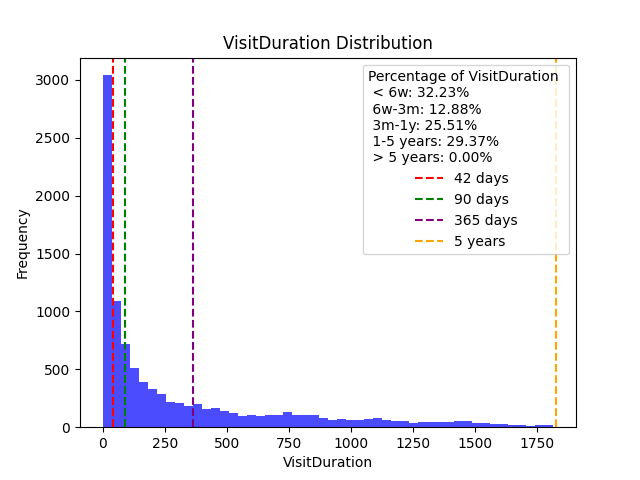
\includegraphics[width=0.8\linewidth]{figures/outcome_distribution.png}
    \caption{Distribution of visit duration in the dataset. The x-axis represents the visit duration in days, and the y-axis represents the number of patients. lines with different colors represent different cutoffs of visit duration. The percentage of patients within different cutoffs are shown in the legend.}\label{visit_duration}
\end{figure}


\subsection{Patient characteristics}\label{PatientCharacteristics}


Of 9921 patients recruited for this study, 3954 patients were selected for time-independent dataset and 1948 patients were selected for time-dependent dataset, the rest were excluded due to serious missing data as describes in methods section. Two datasets were allocated into seperate derivation and external validation sets with a ratio of 7:3, respectively. The comparison of demographic and clinical variables among the training and external validation sets is shown in Table \ref{tab:train_test_origi} for time-independent dataset and Table \ref{tab:train_test_time} for time-dependent dataset. No substantial differences were observed between the training set and the external test set across the majority of features in either time-independent or time-dependent data. Details of the study design are displayed in Figure \ref{protocol}.

% insert image
\begin{figure}[t]
    \centering
    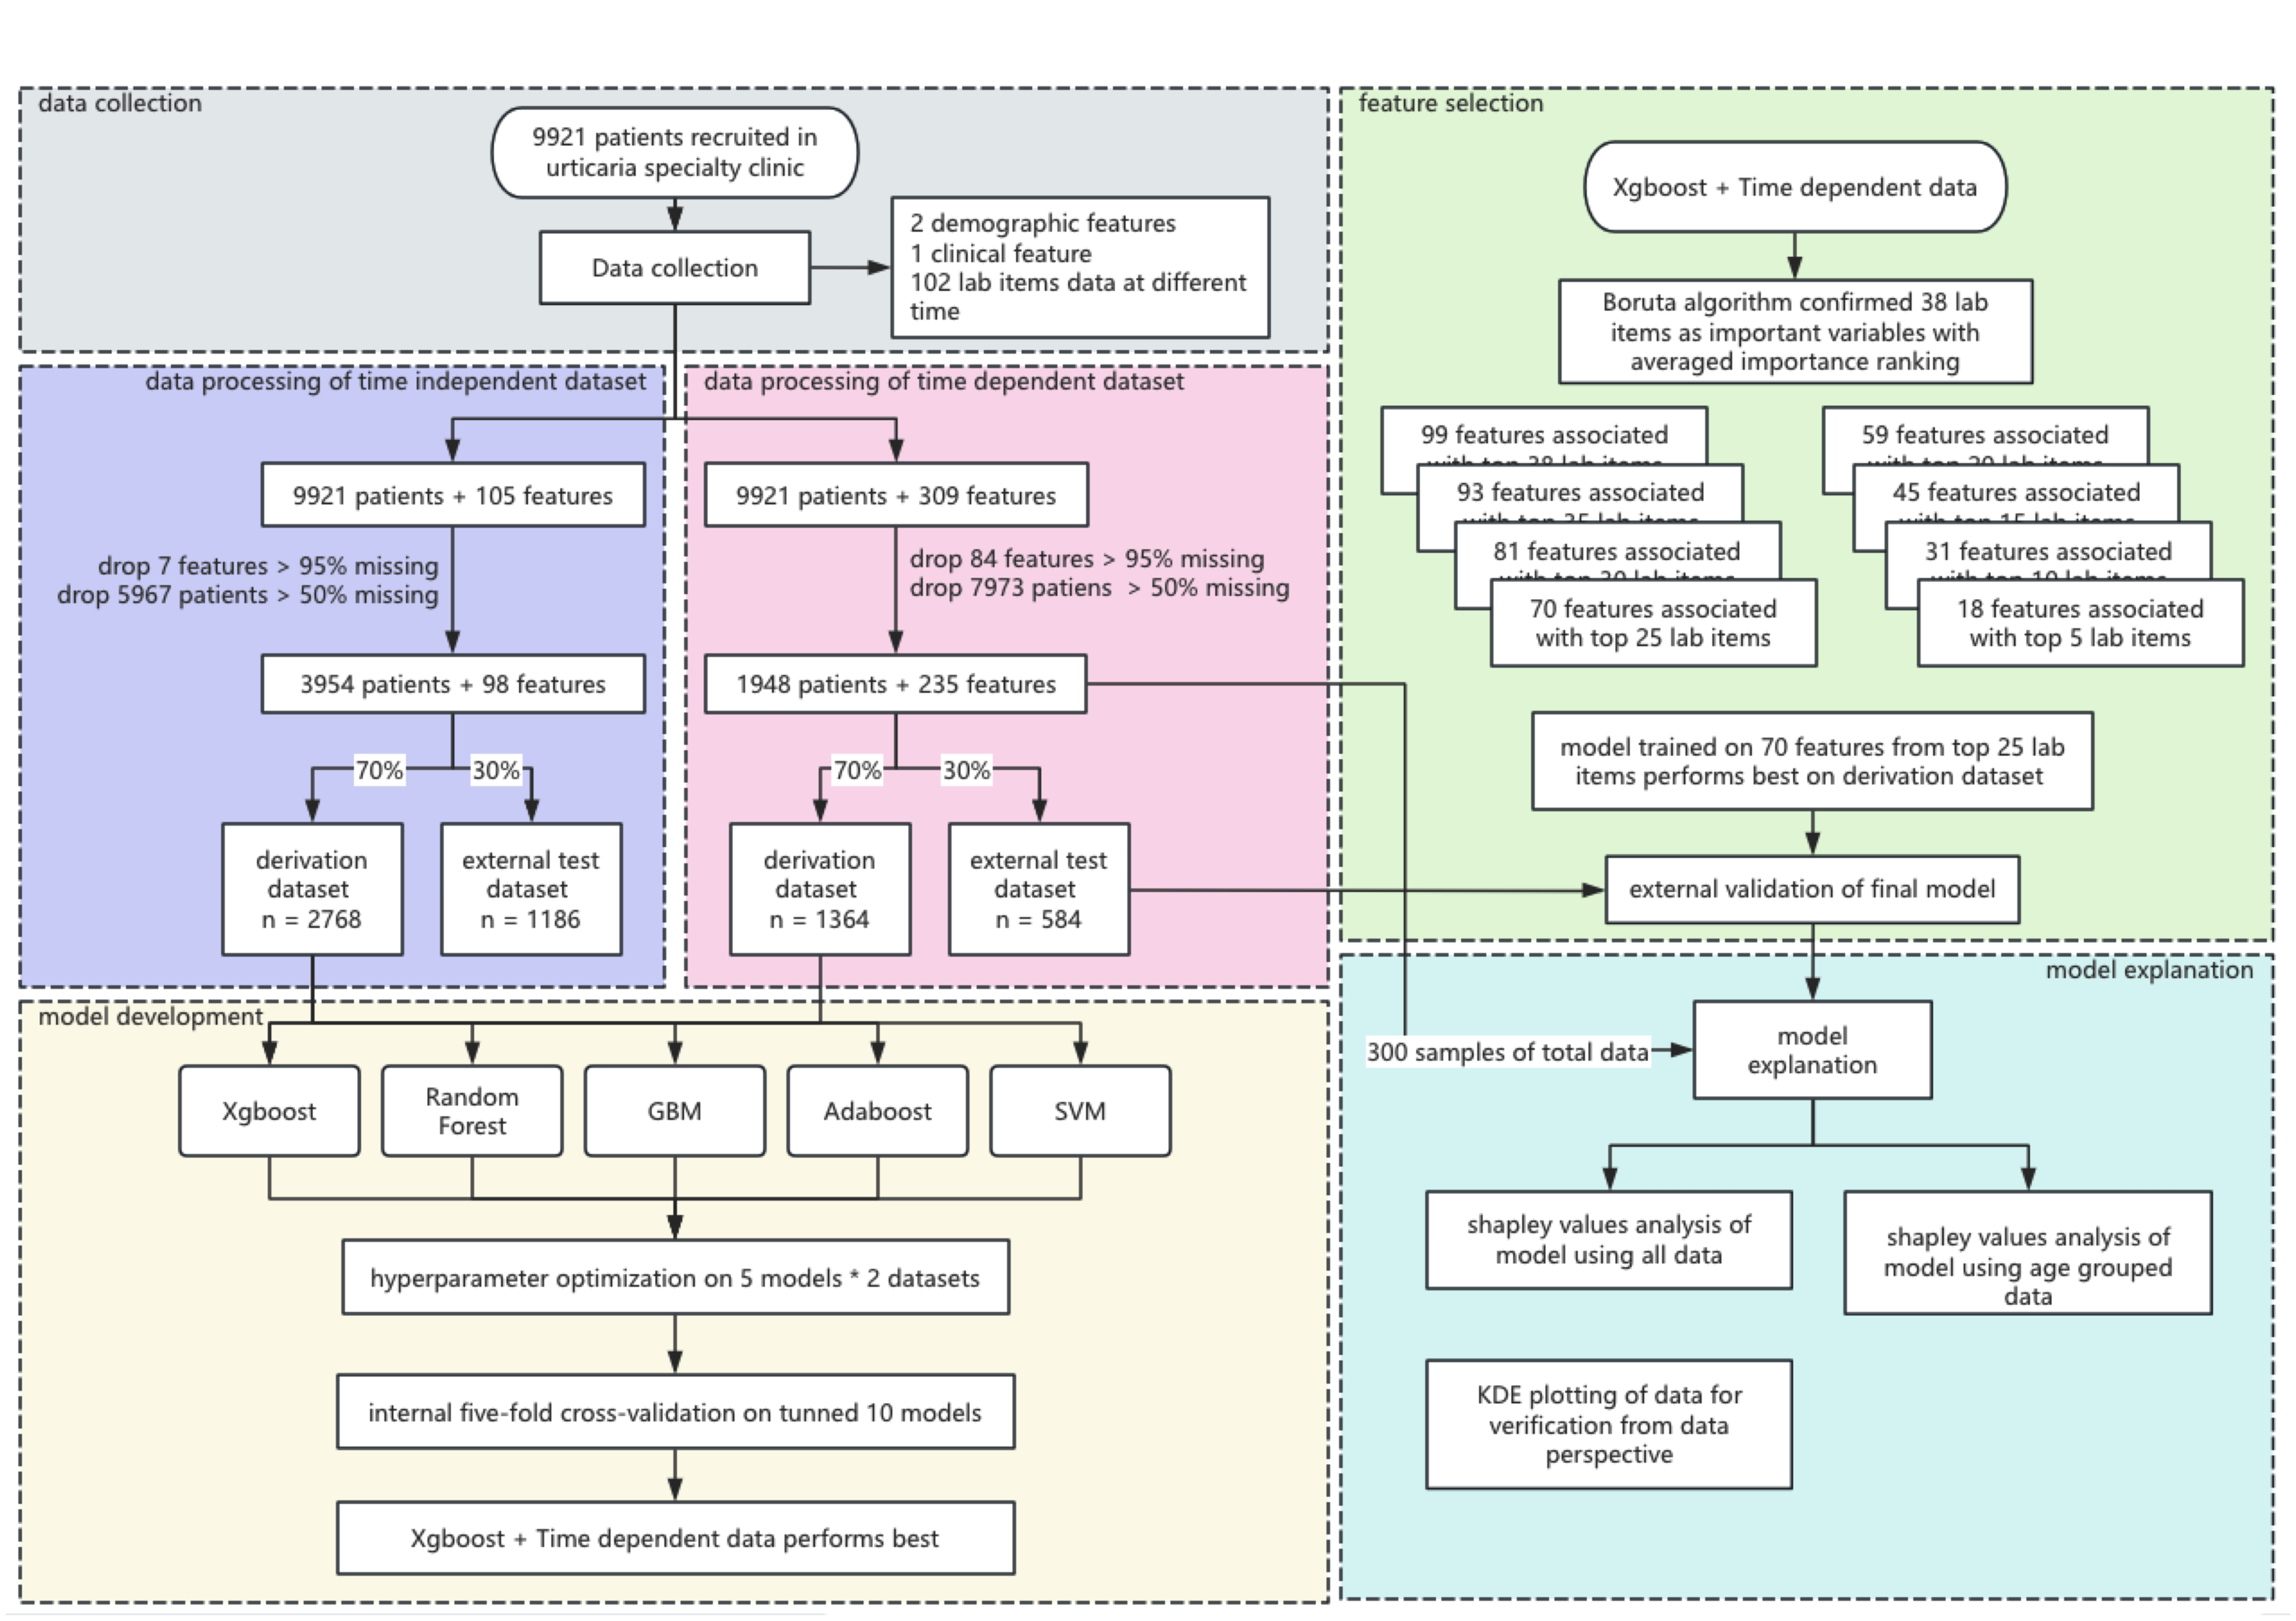
\includegraphics[width=0.8\linewidth]{figures/protocol.png}
    \caption{Study design}\label{protocol}
\end{figure}

The comparison of clinical characteristics between patients with short and prolonged visit duration in the time-independent dataset (Table \ref{tab:good_outcome_poor_outcome_origi}) highlights several trends that align with findings from previous studies on chronic spontaneous urticaria (CSU).
Patients with visiting duration more than 100 days were defined as poor outcome group, and patients with visiting duration less than 100 days were defined as good outcome group. In this analysis, immunoglobulin E (IgE) ($131.65 \pm 242.00$ in good outcome vs $152.28 \pm 346.75$ in poor outcome), and basophil percentage ($0.25 \pm 0.22$ in good outcome vs $0.32 \pm 0.24$ in poor outcome) were significantly higher in patients with poor outcomes, which is consistent with previous studies that have linked these markers to CSU severity and duration \citep{SanchezBorges2017Factors,Rabelo-Filardi2013Parameters}. 

In contrast, C-reactive protein (CRP) levels were significantly lower in patients with poor outcomes ($13.03 \pm 19.62$ in good outcome vs $7.71 \pm 10.23$ in poor outcome), which contradicts previous findings that have associated higher CRP levels with CSU severity \citep{Rabelo-Filardi2013Parameters}. However, this discrepancy could reflect the complexity of CRP as an inflammatory marker that may vary across different disease stages or subgroups of patients. In time-dependent data, which is shown in supplementary Table \ref{tab:good_outcome_poor_outcome_time}, CRP presented various trends in different phases of disease, with significantly lower CRP levels in acute phase ($10.21 \pm 10.95$ in good outcome vs $8.95 \pm 8.22$ in poor outcome) and higher CRP levels in chronic phase ($5.39 \pm 4.84$ in good outcome vs $6.47 \pm 8.81$ in poor outcome) in patients with poor outcomes. This finding suggests that the predictive ability of CRP may be influenced by the disease phase, which could explain the inconsistent results observed in the time-independent dataset.


\begin{table}[htbp]\centering\begin{tabular}{lccc}\hline
    Characteristic & Good Outcome & Poor Outcome & P-value \\
    \hline
    Number of patients & 2027 & 1927 & \\
    
    \makecell[l]{Outcome} & $25.37 \pm 25.09$ & $604.32 \pm 437.04$ & 0.000 $\uparrow$ \\
    
    \makecell[l]{Gender} & 0: 64.7\%, 1: 35.3\% & 0: 61.1\%, 1: 38.9\% & 0.023  \\
    
    \makecell[l]{First Visit Age} & $30.12 \pm 21.79$ & $28.11 \pm 23.61$ & 0.005 $\downarrow$ \\
    
    \makecell[l]{CI nd U} & 0: 99.3\%, 1: 0.7\% & 0: 97.2\%, 1: 2.8\% & 0.000  \\
    
    \makecell[l]{Lymphocytes Percentage} & $28.98 \pm 14.05$ & $34.02 \pm 13.88$ & 0.000 $\uparrow$ \\
    
    \makecell[l]{Neutrophils Percentage} & $63.13 \pm 15.68$ & $56.63 \pm 14.97$ & 0.000 $\downarrow$ \\
    
    \makecell[l]{Monocytes Percentage} & $6.18 \pm 1.64$ & $6.49 \pm 1.67$ & 0.000 $\uparrow$ \\
    
    \makecell[l]{Mean Corpuscular \\ Hemoglobin \\ Concentration} & $335.62 \pm 10.51$ & $336.93 \pm 10.30$ & 0.000 $\uparrow$ \\
    
    \makecell[l]{Platelet Count} & $263.47 \pm 74.09$ & $256.73 \pm 68.96$ & 0.003 $\downarrow$ \\
    
    \makecell[l]{White Blood Cell Count} & $10.31 \pm 3.00$ & $9.35 \pm 2.39$ & 0.000 $\downarrow$ \\
    
    \makecell[l]{Mean Corpuscular \\ Hemoglobin} & $29.07 \pm 2.33$ & $28.98 \pm 2.30$ & 0.202  \\
    
    \makecell[l]{Mean Corpuscular Volume} & $86.66 \pm 6.65$ & $85.99 \pm 6.67$ & 0.002 $\downarrow$ \\
    
    \makecell[l]{Hemoglobin} & $130.03 \pm 9.16$ & $130.20 \pm 8.46$ & 0.546  \\
    
    \makecell[l]{Eosinophils Percentage} & $1.55 \pm 2.02$ & $2.31 \pm 2.37$ & 0.000 $\uparrow$ \\
    
    \makecell[l]{Basophils Percentage} & $0.25 \pm 0.22$ & $0.32 \pm 0.24$ & 0.000 $\uparrow$ \\
    
    \makecell[l]{Absolute Eosinophil \\ Count} & $0.13 \pm 0.20$ & $0.18 \pm 0.21$ & 0.000 $\uparrow$ \\
    
    \makecell[l]{Absolute Lymphocyte \\ Count} & $2.61 \pm 1.12$ & $2.83 \pm 1.29$ & 0.000 $\uparrow$ \\
    
    \makecell[l]{Mean Platelet Volume} & $9.14 \pm 1.39$ & $9.02 \pm 1.39$ & 0.007 $\downarrow$ \\
    
    \makecell[l]{Platelet Distribution \\ Width} & $12.72 \pm 1.96$ & $12.57 \pm 1.94$ & 0.020  \\
    
    \makecell[l]{Eosinophil Count \\ Absolute} & $128.60 \pm 141.68$ & $162.83 \pm 190.02$ & 0.000 $\uparrow$ \\
    
    \makecell[l]{C-reactive Protein} & $13.03 \pm 19.62$ & $7.71 \pm 10.23$ & 0.000 $\downarrow$ \\
    
    \makecell[l]{Immunoglobulin E} & $131.65 \pm 242.00$ & $152.28 \pm 346.75$ & 0.029  \\
    
    \makecell[l]{SMRNP} & $1.18 \pm 2.16$ & $1.22 \pm 1.84$ & 0.576  \\
    
    \makecell[l]{Anti SSA} & $1.42 \pm 5.44$ & $1.58 \pm 5.68$ & 0.363  \\
    
    \makecell[l]{Anti Jo 1} & $1.08 \pm 1.77$ & $1.12 \pm 2.06$ & 0.534  \\
    
    \makecell[l]{Nucleosome} & $0.57 \pm 0.34$ & $0.65 \pm 0.43$ & 0.000 $\uparrow$ \\
    
    \makecell[l]{Ribosomal PP rotein} & $1.07 \pm 0.71$ & $1.17 \pm 2.13$ & 0.050  \\
    
    \makecell[l]{Ro 52} & $2.10 \pm 5.90$ & $2.23 \pm 6.81$ & 0.515  \\
    \hline\end{tabular}\caption{Comparison of the characteristics between patients with good and poor outcomes in the time-independent dataset \\ continuous variables are presented as mean ± standard deviation, categorical variables are presented as number (percentage) \\ good outcome is defined as visit duration < 100 days, poor outcome is defined as visit duration $\geq$ 100 days} \label{tab:good_outcome_poor_outcome_origi}
    \end{table}

\subsection{Comparison of multiple models on time-dependent and time-independent data}\label{ModelComparison}
% xgboost + time-dependent datasset is the best model in 42 100 365 cutoffs

Time-independent and Time-dependent data, combined with 5 different models (XGBoost, Random Forest, AdaBoost, GBM, SVM), were used to generate 10 machine learning models to predict the visiting duration of urticaria. Among the 10 models, the XGBoost model with time-dependent data (AUC = $0.932 \pm 0.016$ for 100, AUC = $0.860 \pm 0.028$ for 365) has the best predictive effect for visiting duration, followed by the Random Forest model with time-dependent data (AUC = $0.922 \pm 0.028$ for 100, AUC = $0.837 \pm 0.037$ for 365) as shown in Figure \ref{kfoldfirst3}. 

Notably, time-dependent data consistently outperformed time-independent data across all models, indicating that the phase-specific laboratory data are more informative for predicting the visiting duration of urticaria. 

The discriminative performances and ROC curves of all 10 models are listed in Supplementary Table \ref{tab:kfold_results}, and Supplementary Figure \ref{fig:kfold_all}, respectively.

% insert image
\begin{figure}[t] 
    \centering 
    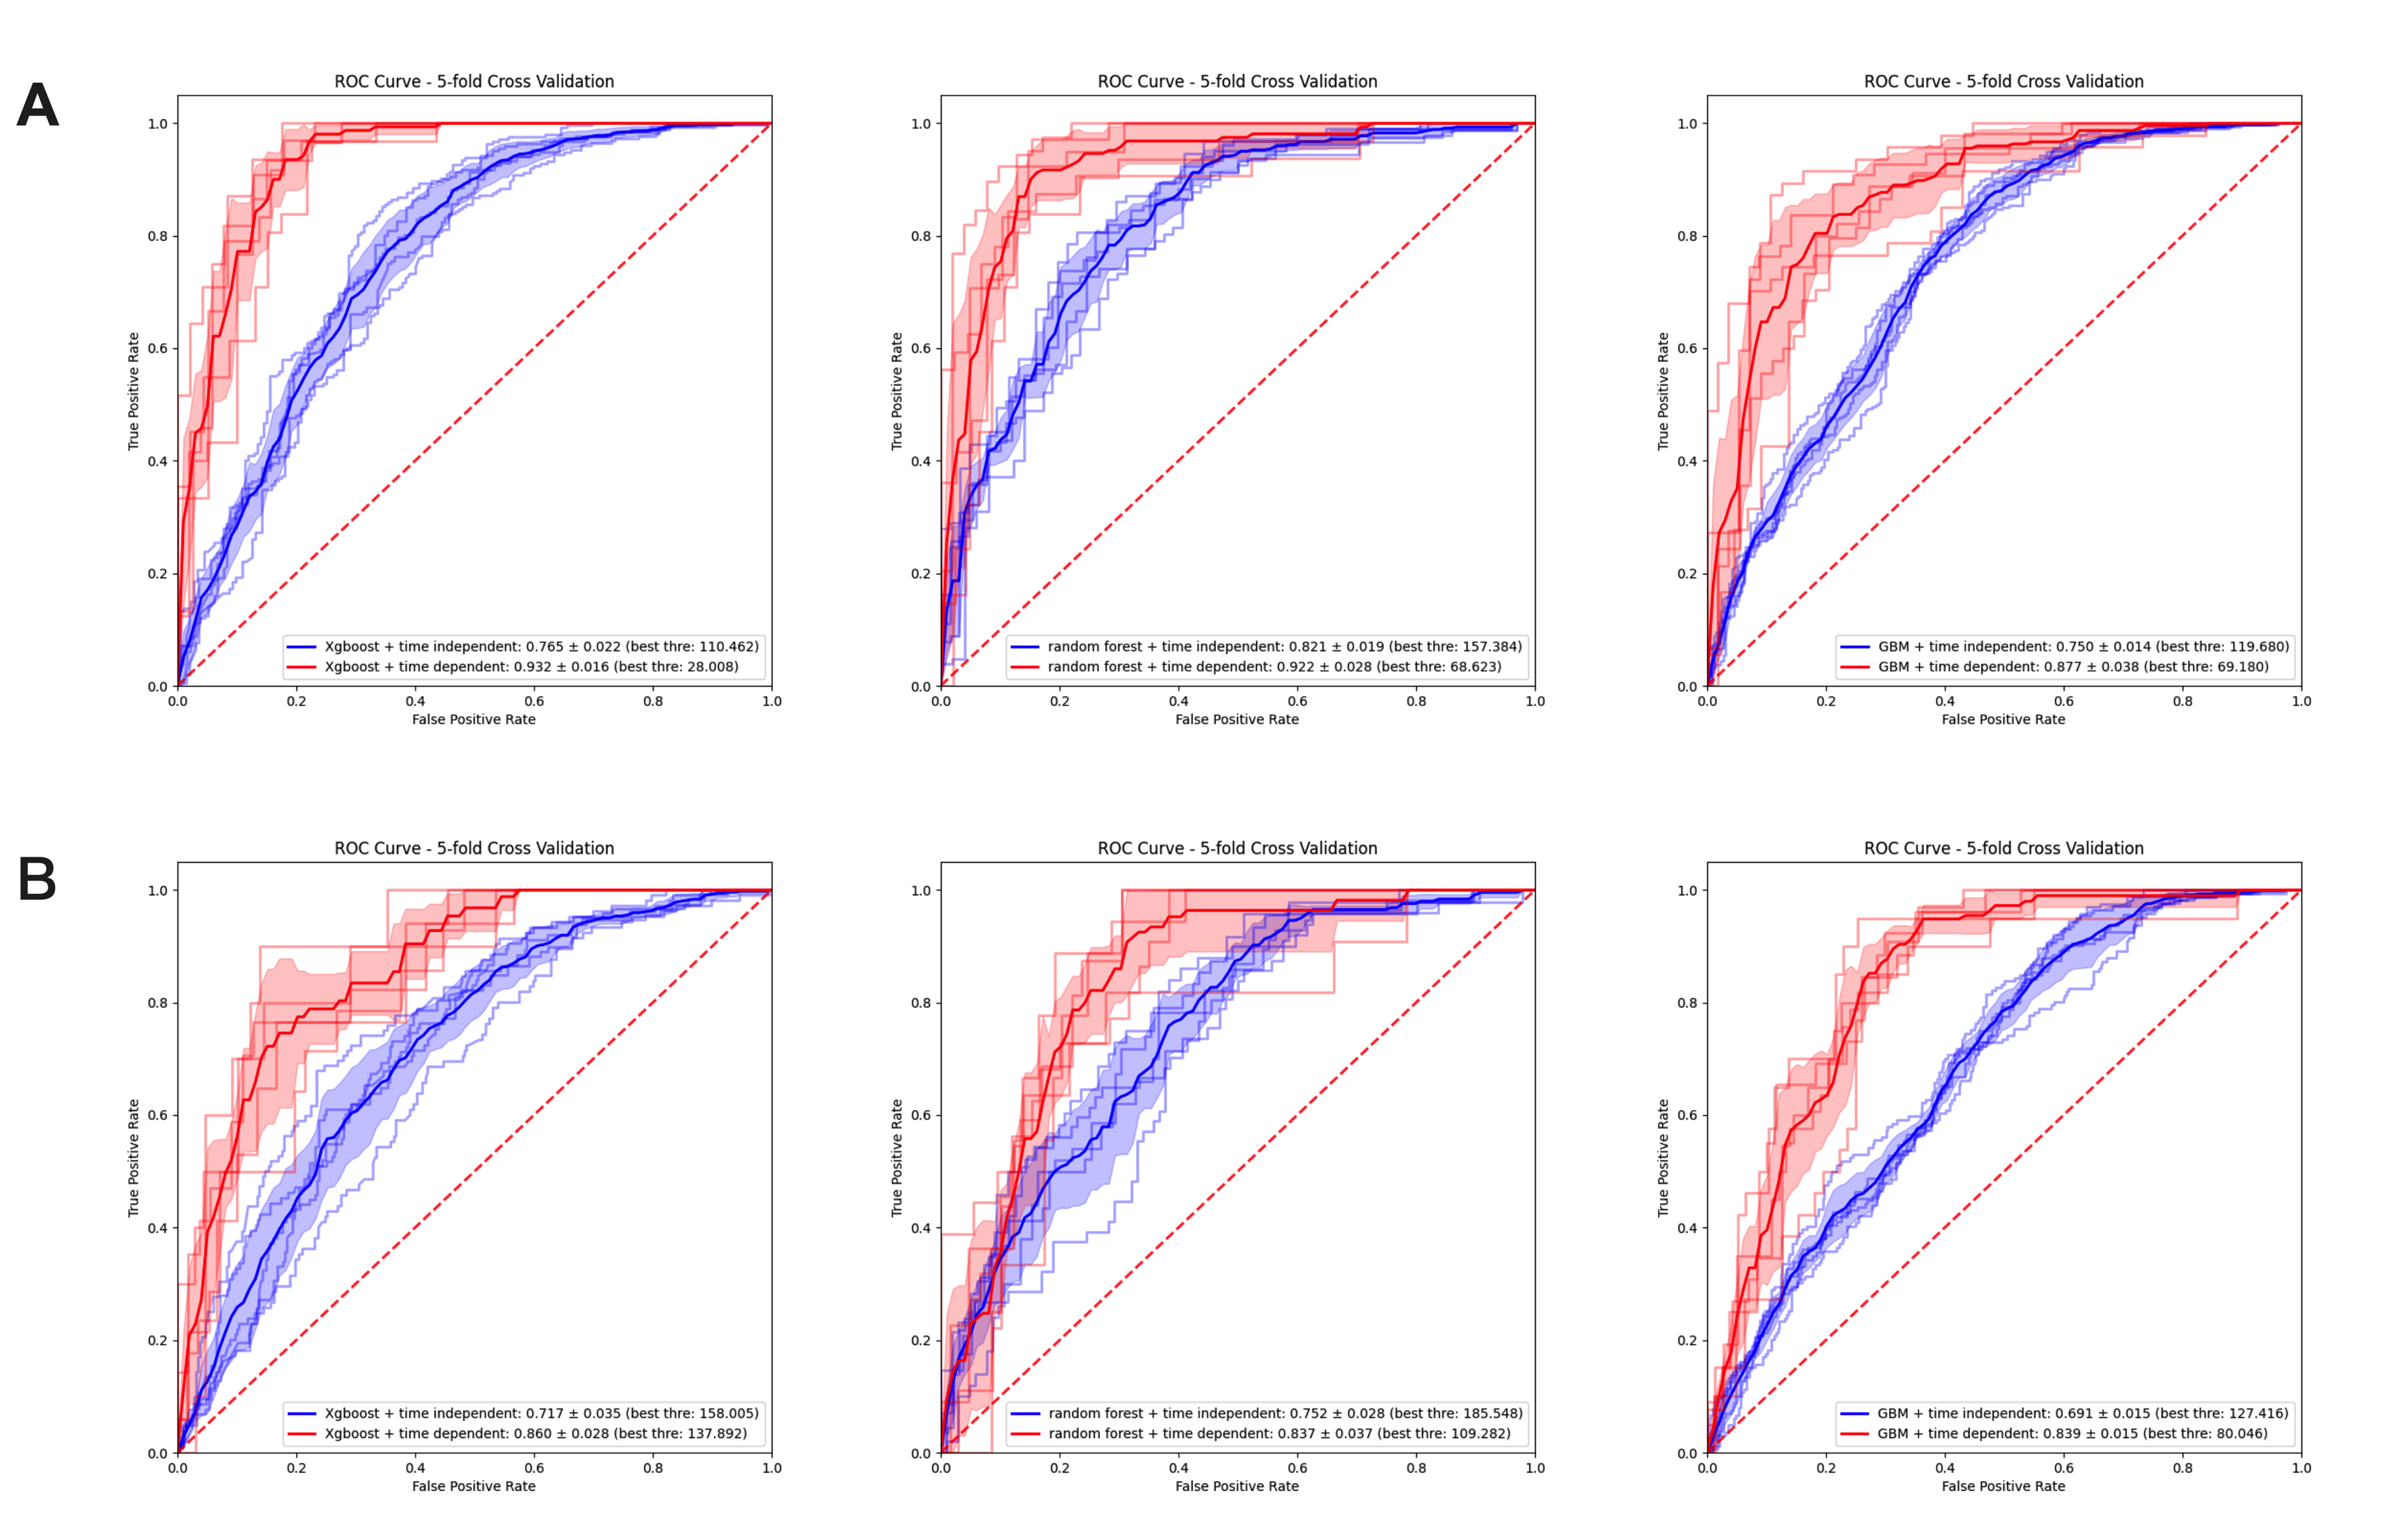
\includegraphics[width=0.8\linewidth]{figures/kfoldfirst3.png} 
    \caption{ROC curves for 5-fold cross-validation results for three different models (XGBoost, Random Forest, and GBM) at 2 binary classification thresholds (100 and 365) in panel A and B. The models' performances are plotted with time-independent and time-dependent datasets, where red indicates the time-independent dataset and blue represents the time-dependent dataset. The shaded areas represent the 95\% confidence intervals.}\label{kfoldfirst3} 
\end{figure}


\subsection{Feature selection and final model}\label{FinalModel}

Xgboost with time-dependent data, as the best performing model, was selected for further optimization. The Boruta algorithm identified 38 laboratory items as important, as shown in Supplementary Table \ref{tab:boruta_confirmed_vars}. Feature importance ranking by Boruta algorithm are shown in Figure \ref{boruta_by_group} and Supplementary Table \ref{tab:boruta_ranking_df}. We rank the confirmed features by the average importance score and compare the model performance on different number of top items.

During the process of reducing features based on the feature importance, the changes in AUCs for the model shows that the model maintain a robust performance unitil the number of items reduced to less than 25, as shown in Figure \ref{topn_extval25} A.

The 25-item model were selected as the final model, and showed a stable performance in external test set with AUC of 0.956 and 0.877 for 100 and 365 cutoffs, as shown in Figure 3 \ref{topn_extval25} B.


% insert image
\begin{figure}[t] 
    \centering
    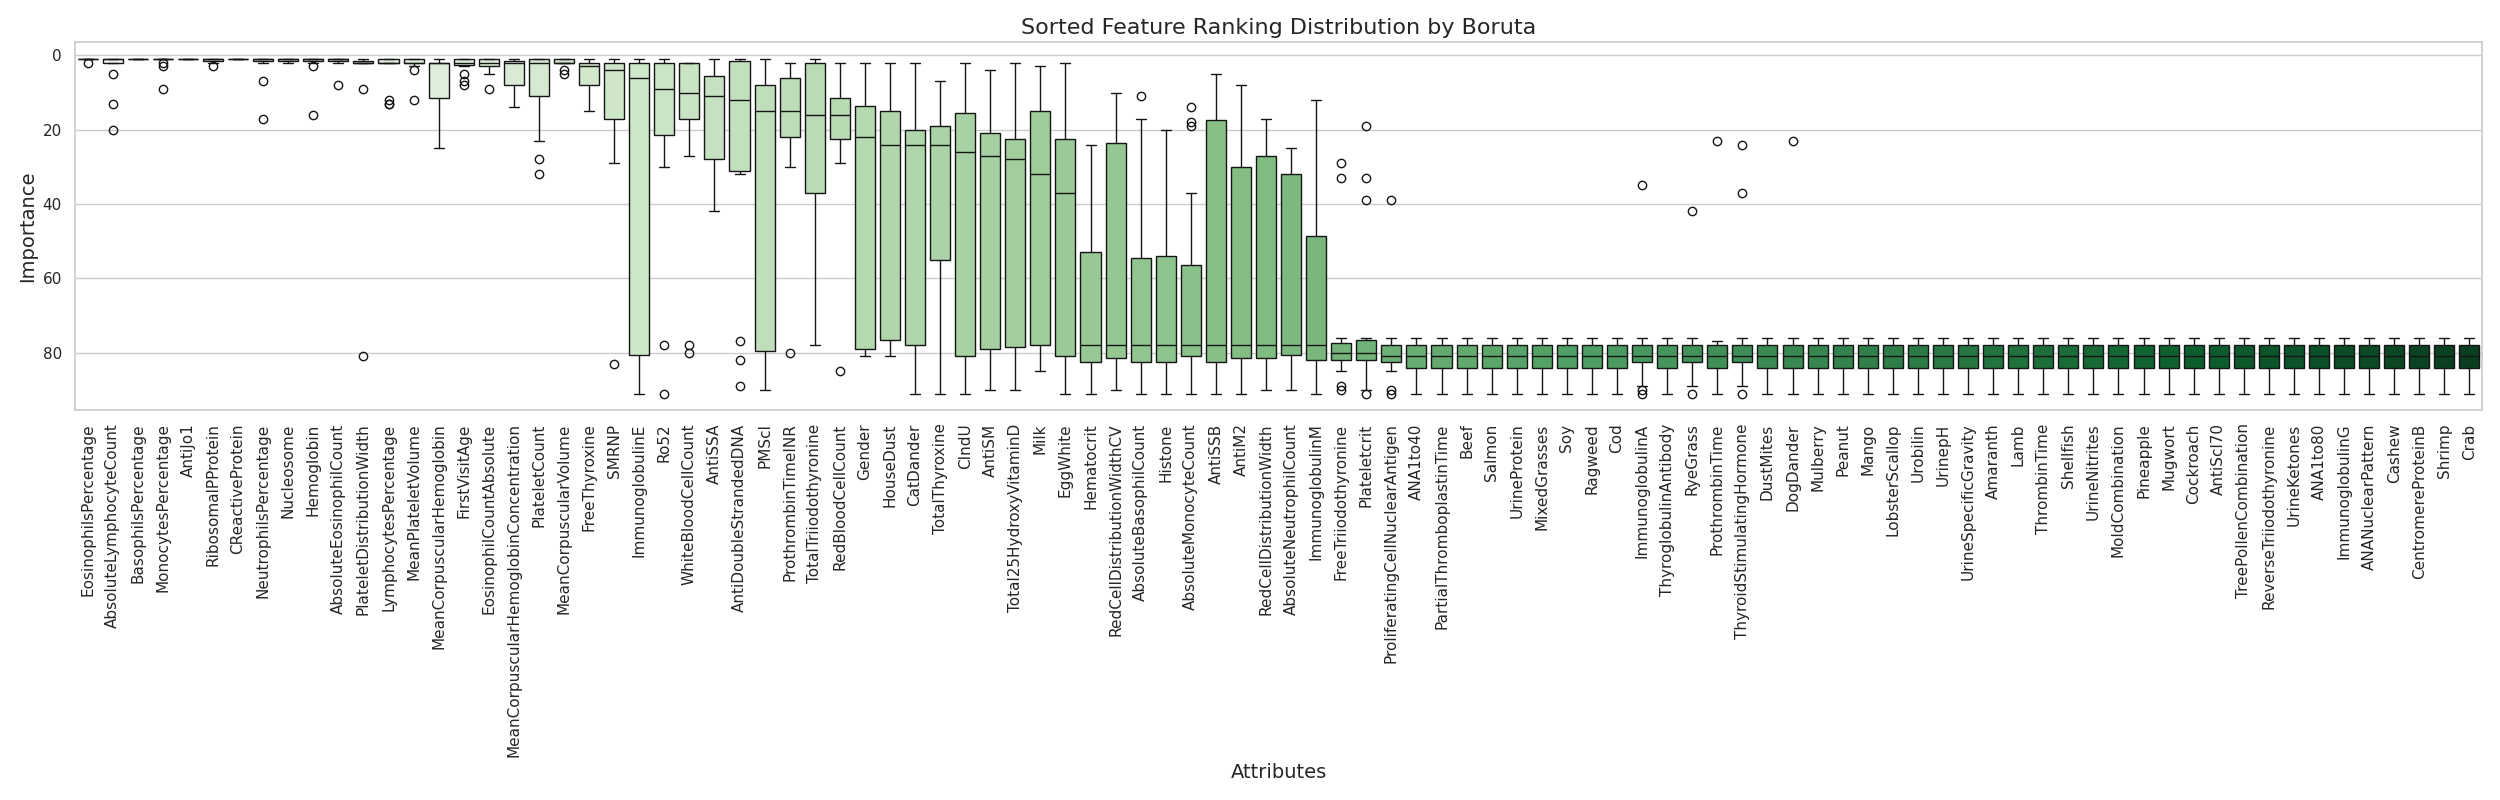
\includegraphics[width=0.8\linewidth]{figures/boruta_by_group.png} 
    \caption{Boxplot representing averaged feature ranking distribution for each laboratory item generated by the Boruta algorithm over 15 iterations. The ranking value for each laboratory item is averaged for 3 different phases of disease. The y-axis shows the importance rank, with lower values indicating higher importance, while the x-axis lists the laboratory items names.}\label{boruta_by_group}
\end{figure}


% insert image
\begin{figure}[t]  
    \centering 
    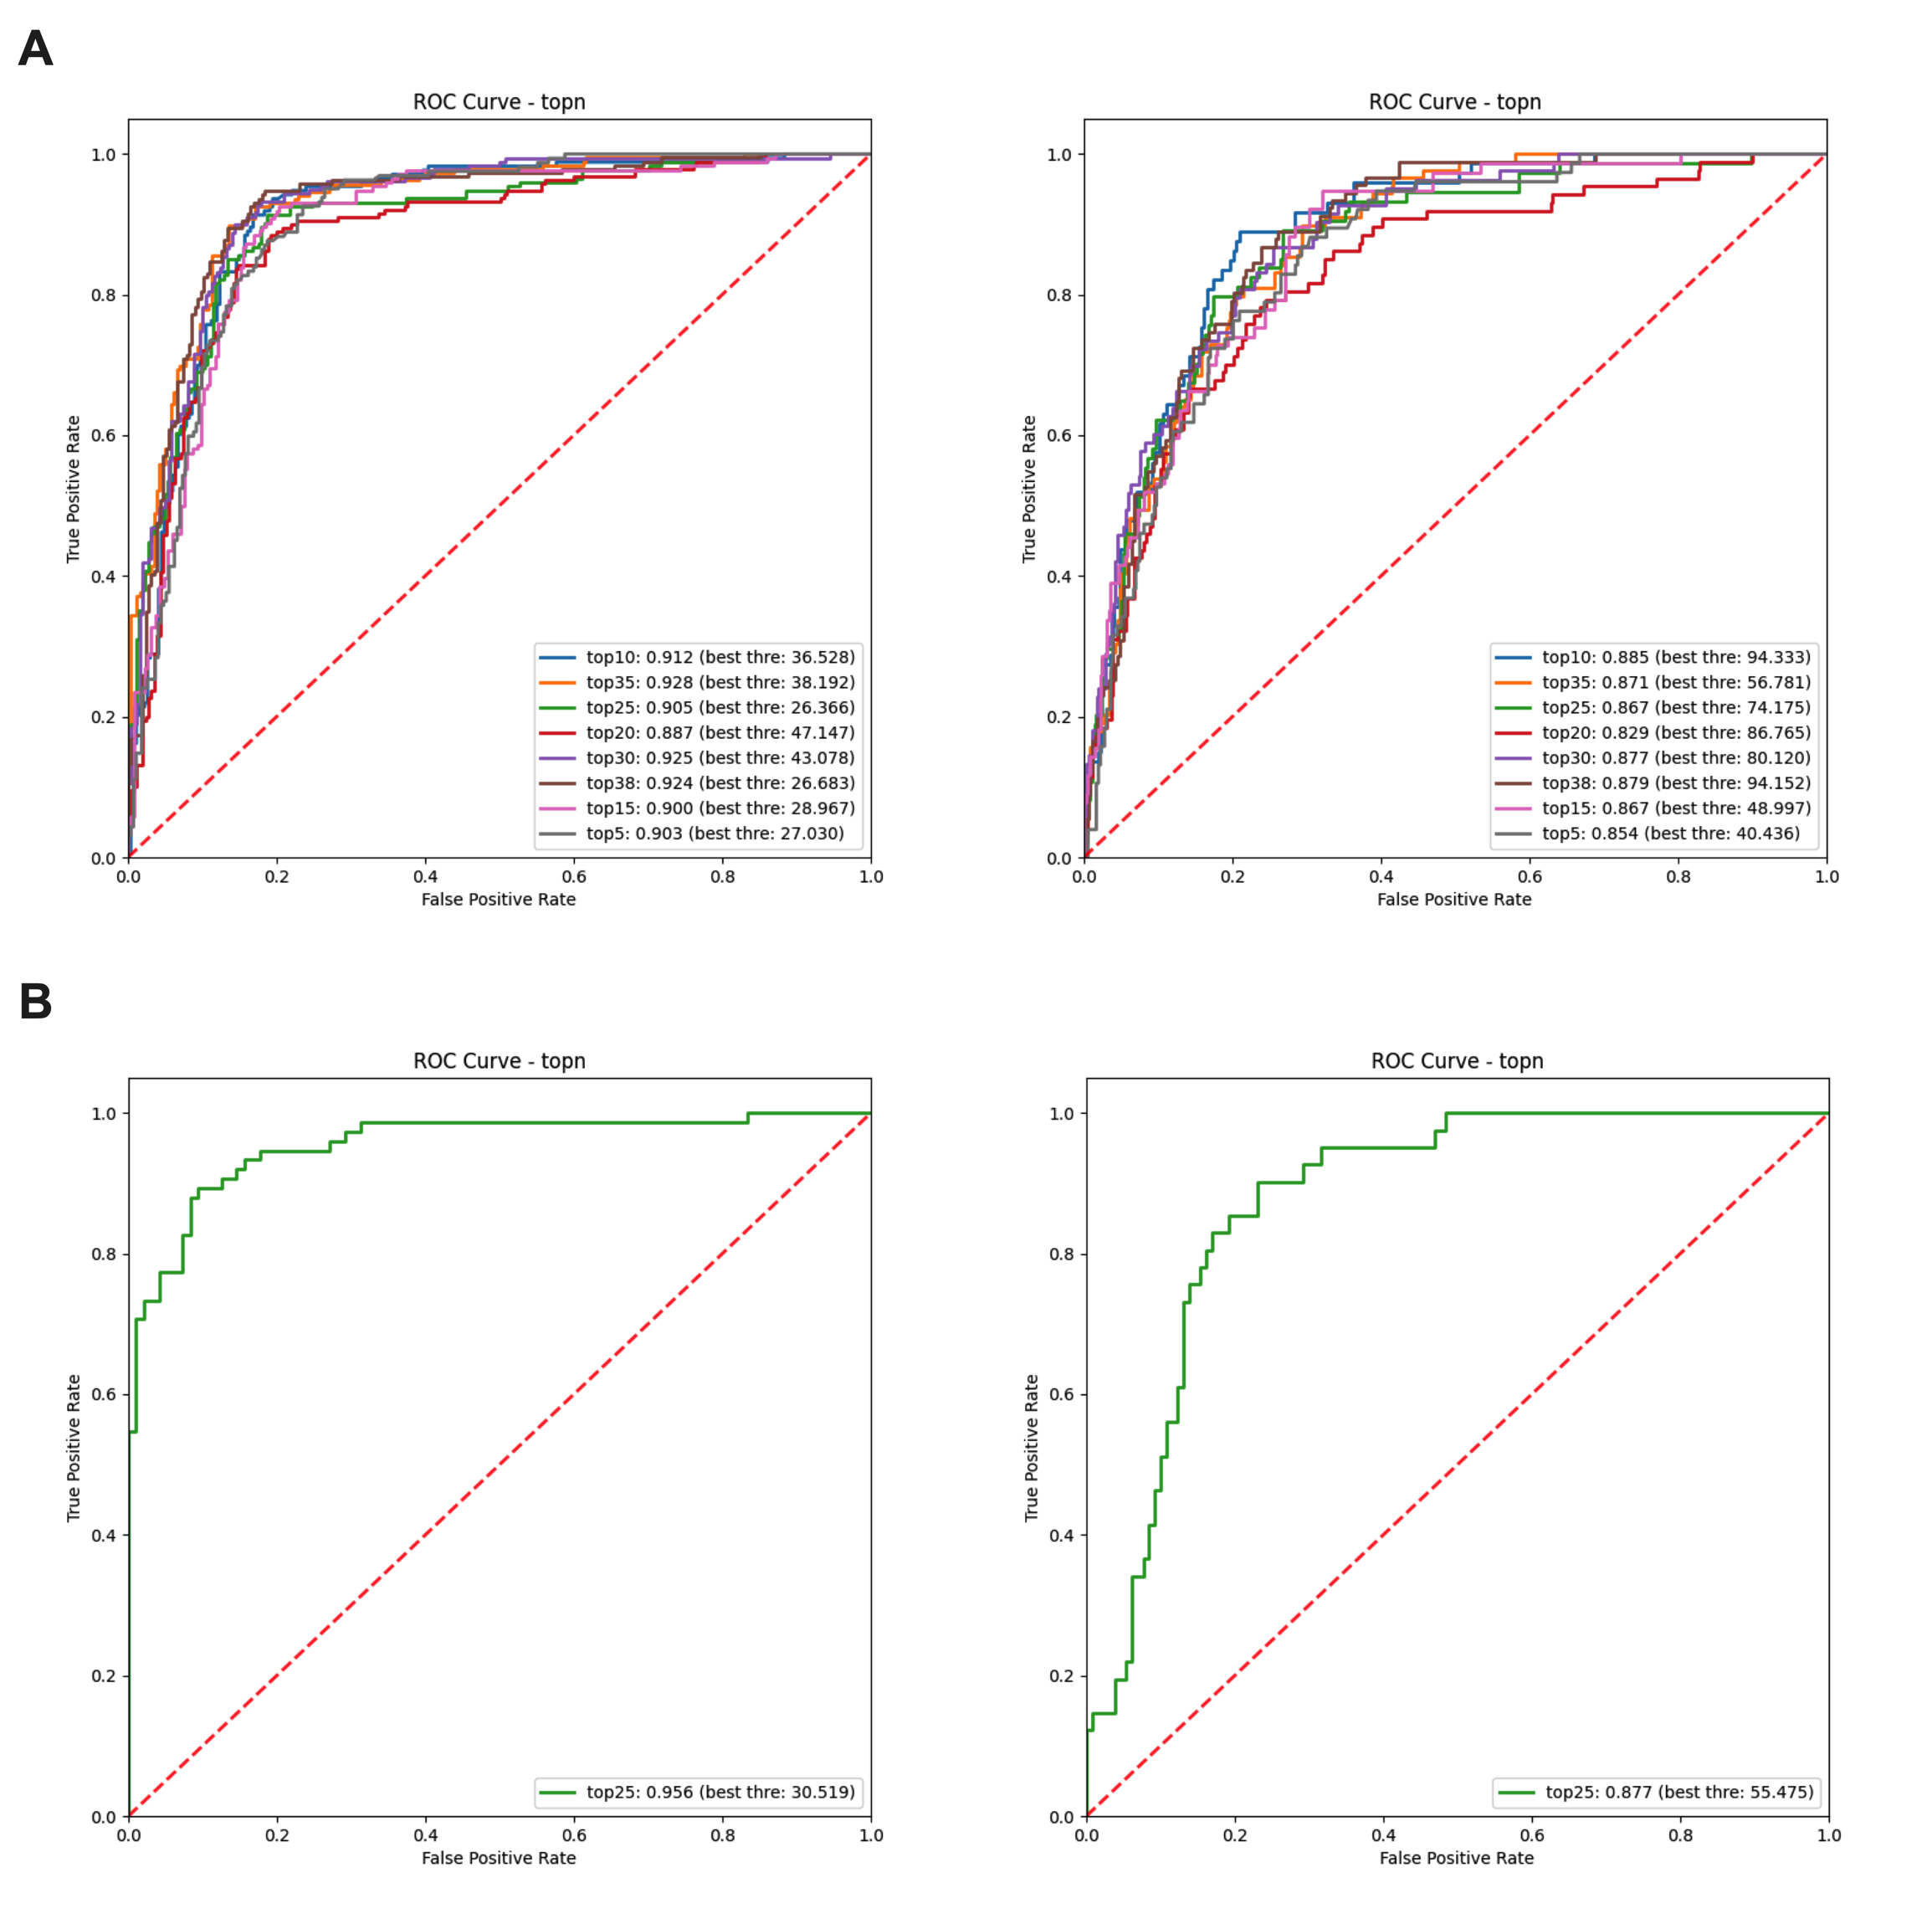
\includegraphics[width=0.8\linewidth]{figures/extvaltopn.png} 
    \caption{Panels A display the ROC curves for the model as the number of top items is reduced based on the average importance score at cutoff values of 100 and 365, respectively. Panels B show the ROC curves for the final model on external test set at cutoff values of 100 and 365, respectively.}\label{topn_extval25}

\end{figure}


\subsection{Model explanation}\label{ModelExplanationResults}
SHAP analysis was conducted on the final model to evaluate the feature importance. Figure \ref{heatmap_all_orderx} presents a heatmap of SHAP values from 100 randomly selected samples, ordered by hierarchical clustering to group similar patterns. The heatmap illustrates how these features influence the model’s output, with global feature importance displayed as a bar plot.

\begin{figure}[t] 
    \centering
    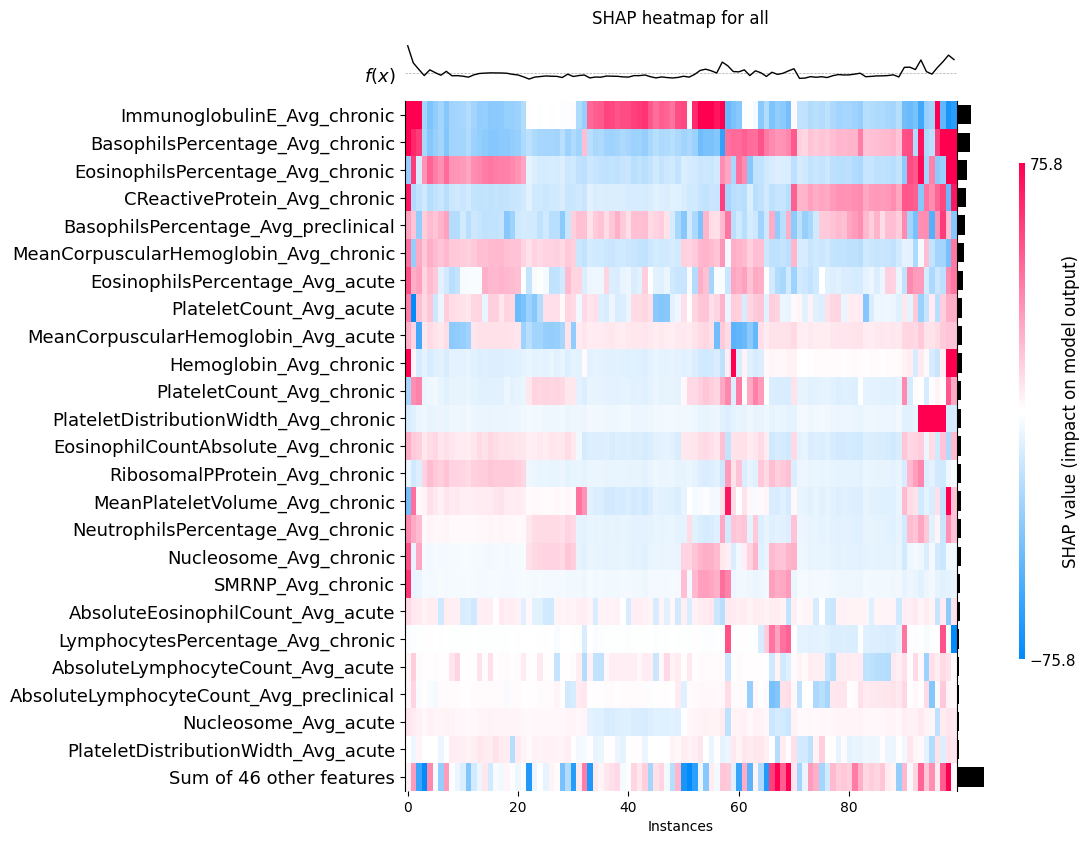
\includegraphics[width=0.8\linewidth]{figures/heatmap_all_orderx.png}
    \caption{a heatmap plot of SHAP values of all features on 100 randomly selected instance, with the instances on the x-axis, the model inputs on the y-axis, and the SHAP values encoded on a color scale. The samples are ordered based on a hierarchical clustering by their explanation similarity. This results in samples that have the same model output for the same reason getting grouped together. The output of the model is shown above the heatmap matrix, and the global importance of each model input shown as a bar plot on the right hand side of the plot.}\label{heatmap_all_orderx}
\end{figure}


\subsubsection{SHAP analysis reveals alignment with previous studies while discovering phase-specific trends}

SHAP analysis on well-known markers of CSU severity and duration, such as eosinophils, basophils, and CRP, revealed consistent trends with previous studies while providing insights on how those markers in different phase can have different predicting ability. 

A high basophil percentage during the chronic phase of the disease pushed the model output towards predicting a longer visit duration. This finding aligns with previous research on chronic spontaneous urticaria (CSU) \citep{SanchezBorges2017Factors}. Interestingly, basophils had no impact in the acute phase and showed a reversed effect during the preclinical phase (Figure \ref{modelexplanation} A). 

A low eosinophil percentage or count consistently pushed the model toward predicting longer visit durations across all disease phases (Figure \ref{modelexplanation} B). This finding is in line with previous studies, which associate eosinopenia with type IIb autoimmunity, heightened disease activity, and poor treatment responses in CSU patients \citep{Kolkhir2019Eosinopenia}.

Lymphocyte percentage and neutrophil percentage in chronic phase also shows harmful effect on patients with longer visit duration, as shown in Figure \ref{modelexplanation} C and D.


High immunoglobulin E levels in the chronic phase of disease was having positive effect on the model output, which is consistent with previous studies that have linked high IgE levels to CSU severity and duration \citep{SanchezBorges2017Factors}, while having no effect in the acute phase of disease, as shown in Figure \ref{modelexplanation} C.

The increasing CRP levels in the chronic phase of disease was having positive effect on the model output, same as the previous studies that have associated higher CRP levels with CSU severity \citep{Rabelo-Filardi2013Parameters}, while the extreme high CRP levels in the acute phase of disease was having negative effect on the model output, as shown in Figure \ref{modelexplanation} B. 

High mean platelet volume was having positive effect on the model output, a trend that was proved by previous studies \citep{Aleem2015Correlation, Magen2010Increased}, while having no effect in the acute and preclinical phase of disease, as shown in Figure \ref{modelexplanation} G.

Thyroid dysfunction is a common comorbidity in patients with chronic urticaria, and it has been reported that reducing thyroxine dose may cause flare-ups of chronic urticaria and angio-oedema, suggesting a possible link between thyroid function and urticaria severity \citep{Dunkley2003Thyroid}. Our study shows that a high TSH level in the chronic phase of disease is having negative effect on the model output, as shown in Figure \ref{modelexplanation} E.

At last, autoimmunity markers, such as Anti Jo 1 and Ro 52, are having positive effect on the model output, as shown in Figure \ref{modelexplanation} I and J.

Other features that were not mentioned in the previous studies, such as mean corpuscular hemoglobin concentration, mean corpuscular volume, and platelet distribution width, also showed significant effects on the model output, as shown in Supplementary Figure \ref{modelexplanation2}.

KDE plots of features mentioned above in different phases of disease are shown in Supplementary Figure \ref{modelexplanation_kde} to illustrate the feature effect from the data perspective.

% insert image
\begin{figure}[t] 
    \centering
    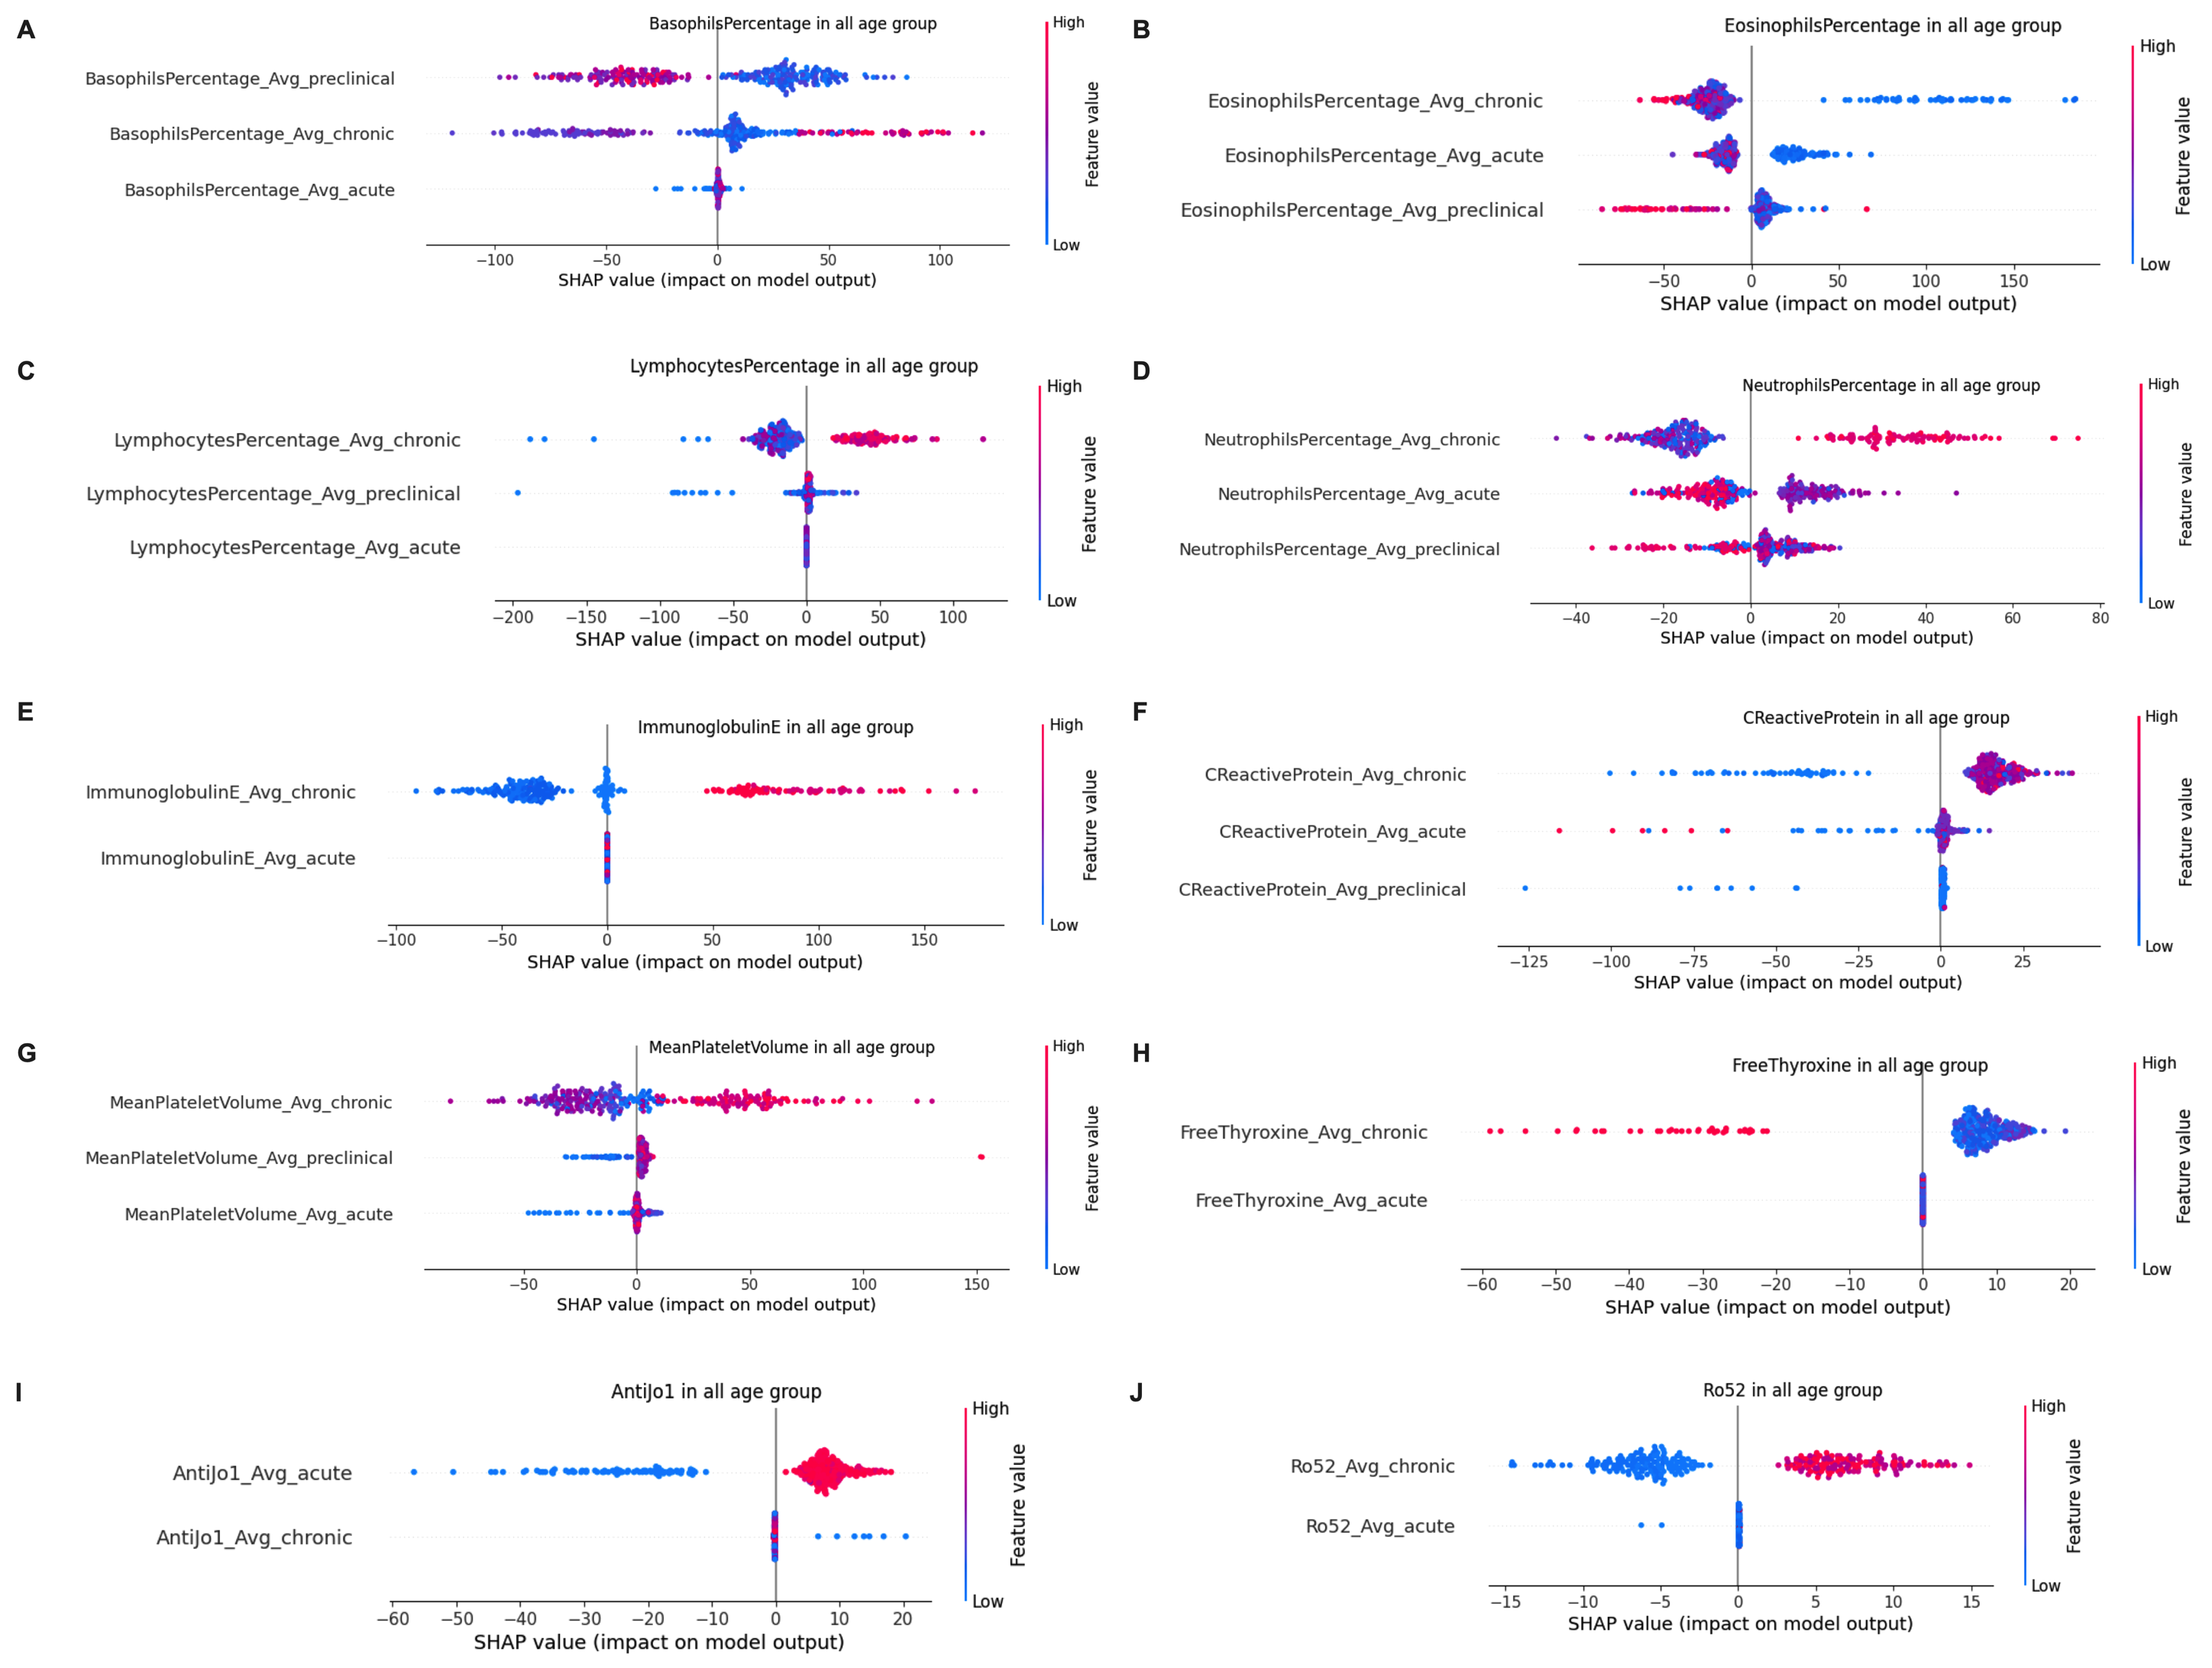
\includegraphics[width=0.8\linewidth]{figures/modelexplanation.png} 
    \caption{SHAP value summary plots for well-known laboratory markers across different disease phases (preclinical, acute, and chronic) in all age groups. Each dot represents a patient sample, with the x-axis indicating the SHAP value (the feature’s impact on the model output) and the color gradient representing the feature value (red for high values, blue for low values). Features with higher SHAP values indicate a greater positive impact on predicting longer visit durations, while negative SHAP values correspond to shorter visit durations.}\label{modelexplanation}
\end{figure}


\subsubsection{SHAP analysis in different age groups shows novel age effect}

Age-specific analysis revealed that the predictive power of laboratory data varies across different age groups. Notably, the absolute eosinophil count in the acute phase had a stronger positive effect on the model’s output for patients aged 0-2, while this effect diminished in patients older than six years (Figure \ref{modelexplanation_age}).

Absolute lymphocyte count also exhibited an age-dependent effect. SHAP analysis showed that a high lymphocyte count during the acute and preclinical phases was beneficial, while it was harmful during the chronic phase. Age subgroup analysis revealed that this predictive trend was significant only in patients older than six years, with little to no effect in younger age groups (Figure \ref{modelexplanation_age2}).
% insert image
\begin{figure}[t]  
    \centering 
    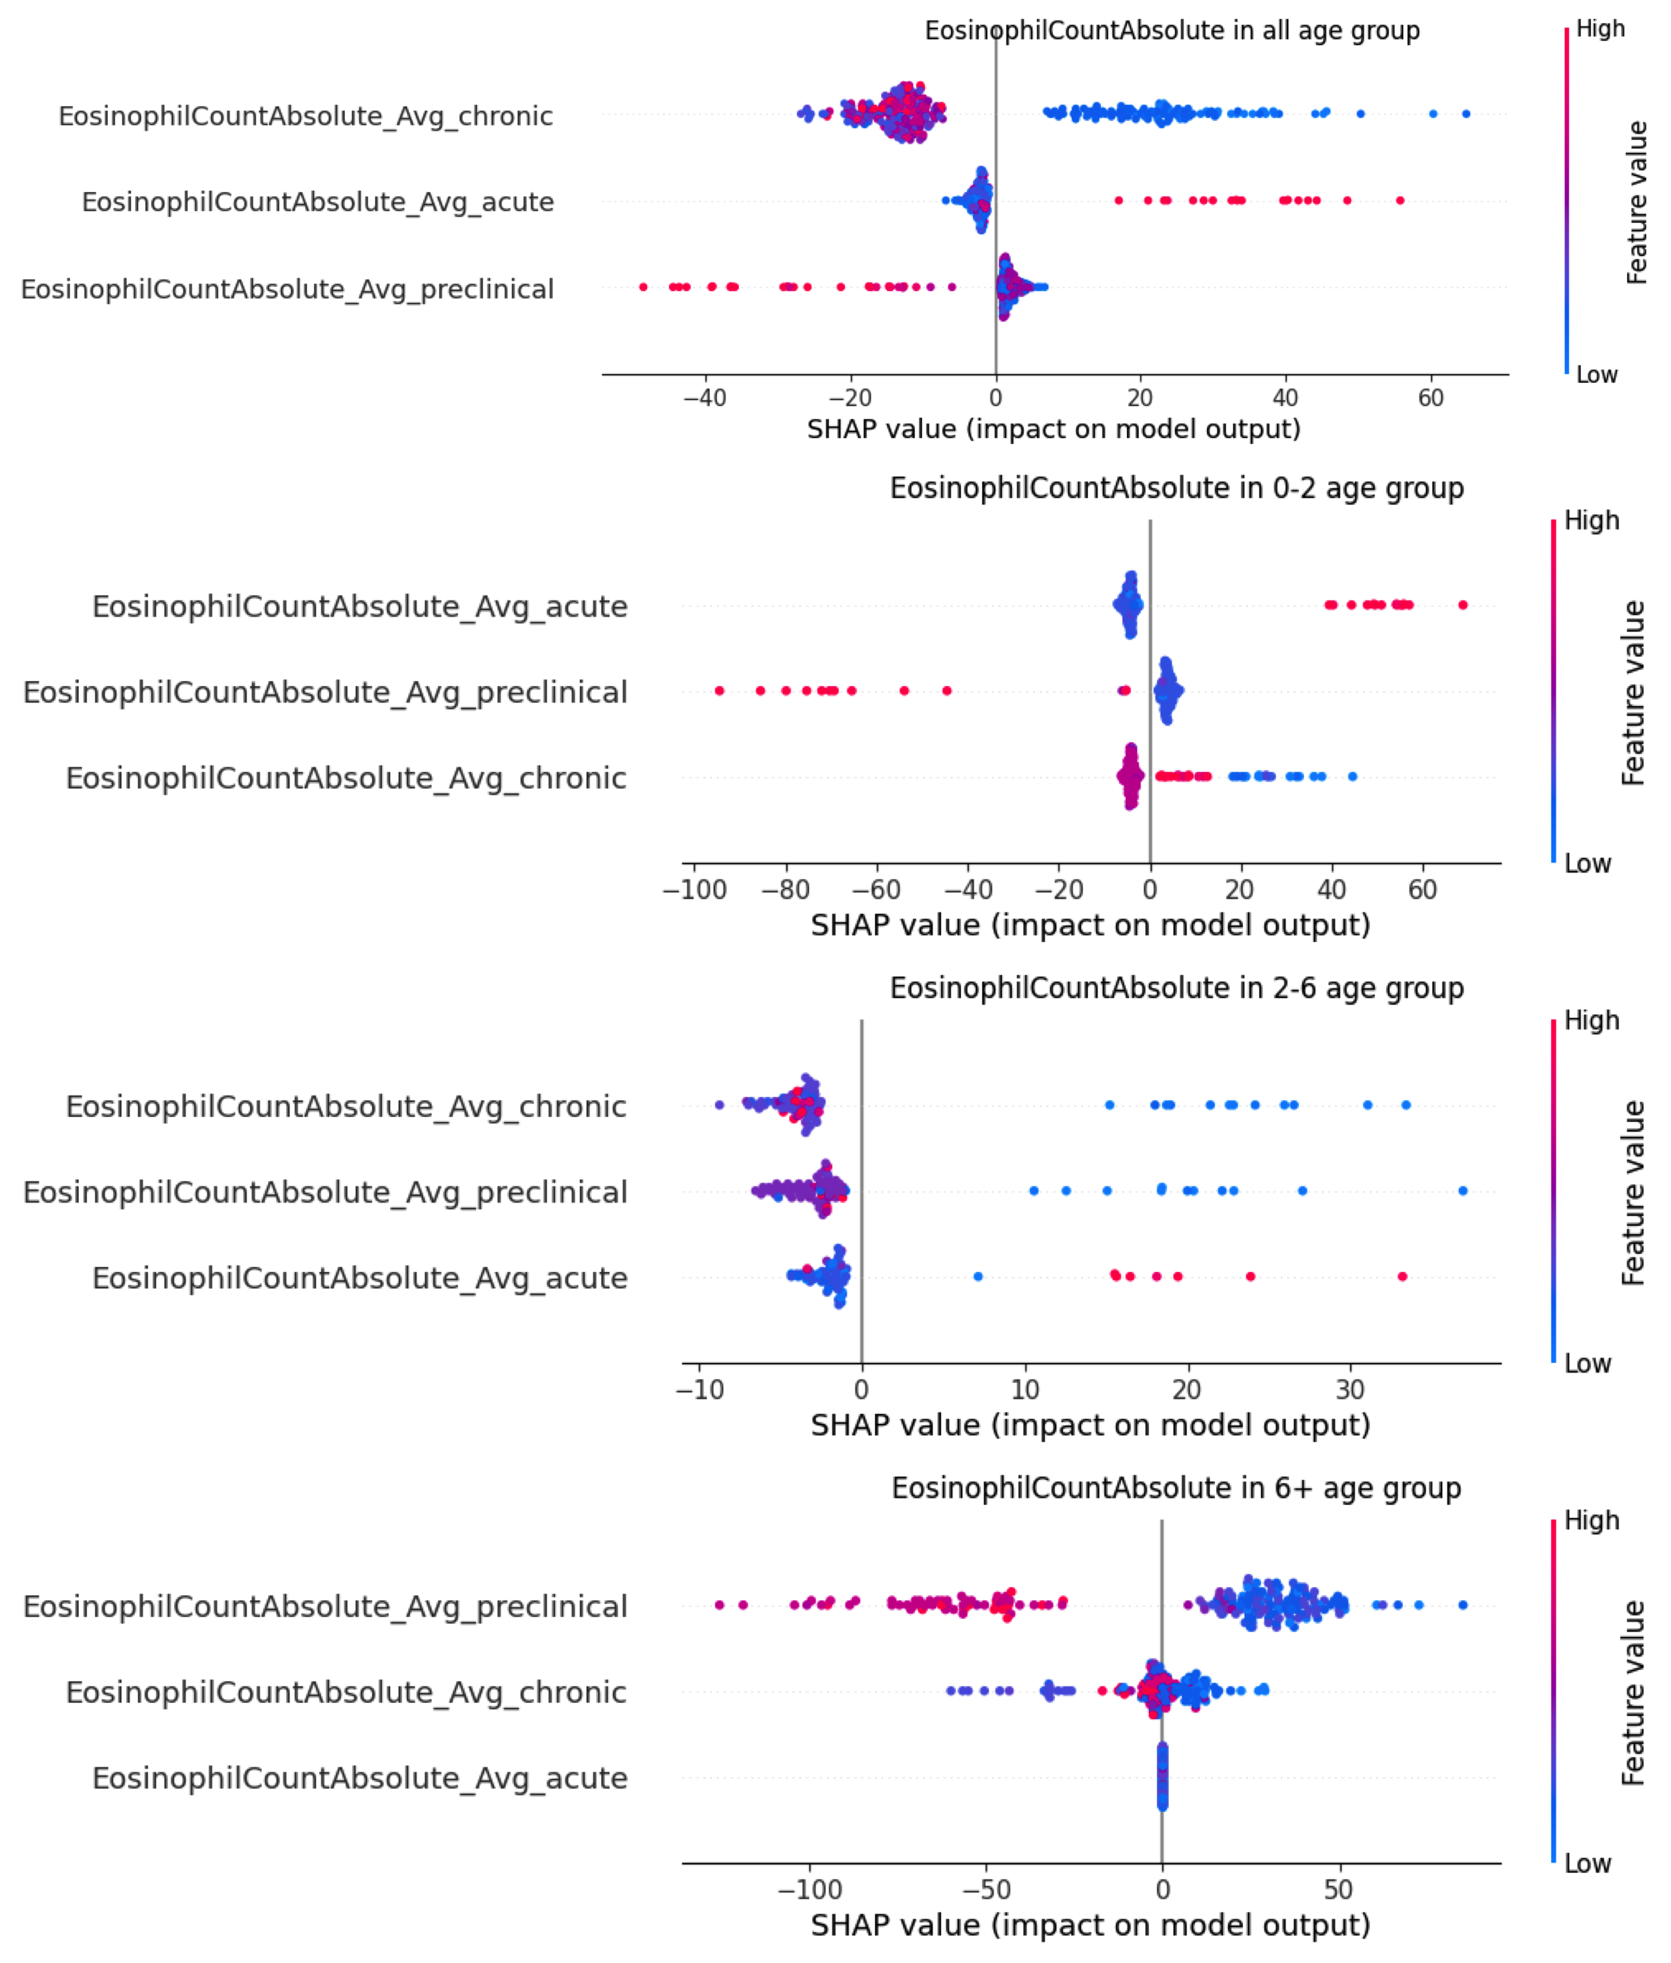
\includegraphics[width=0.5\linewidth]{figures/modelexplanation_age.png}
    \caption{SHAP value summary plots for absolute eosinophil count across different disease phases (preclinical, acute, and chronic) and age groups (all ages, 0-2, 2-6, and 6+ years). Each dot represents a patient sample, with the x-axis indicating the SHAP value (the feature’s impact on the model output) and the color gradient representing the feature value (red for high values, blue for low values).}\label{modelexplanation_age}

\end{figure}


\section{Discussion}\label{Discussion}

% Key Findings and Their Implications
Our study presents several significant findings regarding the prediction of visit duration in patients with chronic spontaneous urticaria (CSU). Utilizing a combination of machine learning models and SHAP analysis, we were able to identify key clinical and laboratory markers that influence disease duration across various phases of CSU. Notably, time-dependent data consistently outperformed time-independent data in predicting visit duration, suggesting that incorporating temporal dynamics provides more nuanced insights into disease progression. Among the models tested, XGBoost with time-dependent data demonstrated the best predictive performance, further highlighting the importance of accounting for longitudinal changes in patient data.

% Predictive Model Performance and Utility
Our comparison of machine learning models demonstrated that the XGBoost algorithm, particularly with time-dependent data, outperformed other models such as Random Forest and GBM. The superior performance of XGBoost can be attributed to its ability to handle non-linear interactions and its robust handling of complex, high-dimensional datasets like those generated in this study. The time-dependent nature of the dataset was particularly important for capturing disease dynamics over time, as patients with CSU often experience fluctuations in their clinical markers and disease activity. This phase-specific approach is crucial, as static time-independent data may overlook these critical variations, resulting in less accurate predictions.

Our findings have significant clinical implications, particularly in the context of personalized medicine. By accurately predicting visit duration based on laboratory and clinical markers, clinicians can better tailor treatment plans, potentially improving patient outcomes. For instance, identifying patients likely to experience prolonged disease duration early in the course of their illness could prompt more aggressive treatment strategies, mitigating disease severity and improving quality of life.

% SHAP Analysis and Clinical Marker Relevance
The SHAP analysis provided valuable insights into the importance of specific laboratory markers in predicting visit duration, revealing both phase-specific and age-specific trends. Key markers such as basophils, eosinophils, and CRP were consistently highlighted across different disease phases, aligning with findings from previous studies on CSU severity and duration \citep{SanchezBorges2017Factors, Kolkhir2019Eosinopenia}.

Basophil percentage, for example, was a strong predictor of longer visit duration in the chronic phase but had no effect in the acute phase and a reversed effect in the preclinical phase. This phase-dependent variation suggests that basophils may play different roles at various stages of the disease, with higher basophil levels potentially indicating a more severe and prolonged disease course in chronic CSU. These findings are consistent with prior research linking elevated basophils to disease severity \citep{SanchezBorges2017Factors}.

Eosinophils also emerged as an important predictor, with low eosinophil percentages or counts correlating with longer disease duration across all phases. Eosinopenia has been associated with type IIb autoimmunity, which is characterized by more severe disease and poorer treatment response in CSU patients \citep{Kolkhir2019Eosinopenia}. This finding reinforces the clinical utility of eosinophils as a biomarker for CSU prognosis.

CRP levels, another well-established inflammatory marker, exhibited complex, phase-specific effects. In the chronic phase, higher CRP levels predicted longer visit durations, consistent with previous studies linking elevated CRP to greater CSU severity \citep{Rabelo-Filardi2013Parameters}. However, in the acute phase, extremely high CRP levels had a negative impact on the model’s predictions, suggesting that CRP’s role as a biomarker may vary depending on the disease stage. This highlights the importance of interpreting inflammatory markers like CRP in the context of disease progression.

% Novel Age-Dependent Effects
In addition to phase-specific trends, our SHAP analysis revealed novel age-dependent effects in the prediction of visit duration. For example, the predictive ability of absolute eosinophil count in the acute phase was more pronounced in younger patients (aged 0-2) but diminished in those older than six years. Similarly, the impact of absolute lymphocyte count was only significant in patients older than six years, suggesting that the immune response in CSU may differ based on age. These findings underscore the need for age-specific considerations when interpreting laboratory data and highlight the potential for more tailored, pediatric-specific treatment strategies in younger CSU patients.

% Comparison with Previous Studies
Our findings build upon and extend previous research on the role of laboratory markers in CSU. Prior studies have identified various biomarkers, such as elevated IgE and eosinophil counts, as indicators of disease severity and duration \citep{SanchezBorges2017Factors, Kolkhir2019Eosinopenia}. However, few studies have explored the phase-specific predictive power of these markers or examined how their relevance may change over the course of the disease. By utilizing SHAP analysis, we were able to uncover these nuanced relationships, demonstrating that certain markers may only be predictive during specific phases of CSU.

Additionally, our study is one of the first to investigate age-dependent effects in CSU biomarker prediction. Previous research has largely focused on adult populations, with little attention given to how biomarkers may function differently in pediatric patients. The age-specific trends we identified offer new avenues for research and suggest that treatment strategies for CSU may need to be adjusted based on patient age.

% Limitations and Future Directions
While our study provides valuable insights into the predictive modeling of visit duration in CSU, several limitations should be acknowledged. First, the lack of patients with visit durations exceeding five years limits the generalizability of our findings to longer-term CSU cases. Future studies should aim to include a broader range of follow-up times to better capture the full spectrum of disease duration. Additionally, while SHAP analysis provides important information about feature importance, it does not establish causality. Further research is needed to explore the mechanistic underpinnings of the relationships we observed between laboratory markers and CSU duration.

Another limitation is the exclusion of patients with missing data, which may have introduced selection bias. Future research should investigate methods for handling missing data, such as multiple imputation, to ensure that results are generalizable to a broader population of CSU patients.

Finally, while our study focused on laboratory markers, future studies should consider incorporating additional clinical data, such as treatment response and comorbidities, to further improve model accuracy and clinical applicability.

% Conclusion
In summary, our study highlights the utility of machine learning models, particularly XGBoost, in predicting visit duration in CSU patients. Time-dependent data proved to be critical in capturing the dynamic nature of the disease, while SHAP analysis revealed phase-specific and age-dependent trends in key laboratory markers. These findings not only enhance our understanding of CSU pathophysiology but also have practical implications for personalized treatment strategies. Future research should continue to explore the use of machine learning and longitudinal data in chronic disease management to further optimize patient care.

% Although the pathogenesis of CSU is not yet fully understood, it is well established that its signs and symptoms are due to the activation of mast cells and basophils, leading to the release of histamine and other inflammatory mediators\citep{Zuberbier2021The}. Based on recent evidence, it is known that the causes of CSU include autoimmunity Type I (CSUaiTI, or “autoallergic CSU”; with IgE autoantibodies to self-antigens) and autoimmunity Type IIb (CSUaiTIIb; with mast cell–directed activating autoantibodies). In CSU due to unknown cause (CSUuc), as of yet unknown mechanisms are relevant for the degranulation of skin mast cell (MC)\citep{sella2023type, Maronese2023IgG}. The results of the basic tests performed in CSU can point to CSUaiTI vs CSUaiTIIb, with CRP more often elevated and eosinophil and basophil levels more often reduced in CSUaiTIIb\citep{Xiang2023Chronic}.


% Eosinopenia in chronic spontaneous urticaria patients is associated with type IIb autoimmunity, high disease activity, and poor treatment response. \citep{Kolkhir2019Eosinopenia}, especially in children \citep{A2023Serum}.

% Acute urticaria patients have abnormal cell immune responses, with lower numbers of CD3+ and CD4+ lymphocytes compared to healthy controls.\citep{De-yu2009Determination}.

% Chronic idiopathic urticaria is associated with a prominent infiltrate of T-lymphocytes, monocytes, and mast cells, suggesting potential interactions between these cells to cause mediator release.\citep{Elias1986Studies}

% Reducing thyroxine dose may cause flare-ups of chronic urticaria and angio-oedema, suggesting a possible link between thyroid function and musculoskeletal conditions.\citep{Dunkley2003Thyroid}

% Mean platelet volume levels are higher in patients with chronic urticaria and correlate with its severity, suggesting coagulation and inflammation may play a role in the disease.\citep{Aleem2015Correlation} Chronic urticaria with a positive autologous serum skin test is associated with higher clinical severity, increased platelet volume, and increased C-reactive protein levels.\citep{Magen2010Increased} 

% Neutrophilic urticarial dermatosis is a distinct cutaneous manifestation of neutrophilic aseptic disease, strongly associated with systemic diseases like Schnitzler syndrome, adult-onset Still disease, lupus erythematosus, and hereditary autoinflammatory fever syndromes.\citep{Kieffer2009Neutrophilic} Neutrophilic urticaria is common and not associated with other diseases, but its presence in biopsy samples may indicate rheumatic disease.\citep{Llamas‐Velasco2012Neutrophilic}


% Omalizumab treatment significantly reduced neutrophil\/lymphocyte ratio and neutrophil\/monocyte ratio in patients with chronic spontaneous urticaria\citep{Maurer2015Management}. Neutrophils can serve as antigen-presenting cells for local allergen-specific effector T cells in patients with allergic late-phase reactions\citep{Polak2019A}.


% The SHAP analysis performed in this study provides valuable insights into the prediction of visit duration for chronic spontaneous urticaria (CSU) based on clinical laboratory data, aligning with previous studies while also revealing novel findings. Consistent with prior research, our model demonstrates that elevated basophil percentages during the chronic phase of CSU are associated with longer visit durations, in line with previous findings \citep{SanchezBorges2017Factors}. Similarly, increased CRP levels during the chronic phase were found to have a positive effect on the model's output, corroborating earlier studies that have linked higher CRP levels with CSU severity and prolonged visiting duration \citep{Rabelo-Filardi2013Parameters}. However, an unexpected negative effect of extreme CRP levels during the acute phase was identified, indicating that elevated CRP might play a different role in the early stages of the disease. Immunoglobulin E, absolute lymphocytes count, free thyroxine, and mean platelet volume were also found to have significant impacts on the model output, consistent with previous research that has highlighted the importance of these markers in CSU severity and duration \citep{SanchezBorges2017Factors, Aleem2015Correlation, Dunkley2003Thyroid,Magen2010Increased}.

% A novel discovery in our analysis is the phase-specific behavior of certain biomarkers. While a high eosinophil percentage in the preclinical phase was associated with shorter visit durations, the same marker in the chronic phase contributed to prolonged visits, highlighting distinct dynamics depending on the disease stage. Additionally, the SHAP analysis revealed that IgE levels, often associated with CSU severity and duration \citep{SanchezBorges2017Factors}, only had a significant impact during the chronic phase, with no effect in the acute phase. This phase-specific difference in the predictive power of laboratory markers represents a significant innovation in understanding CSU's progression.

% Our study also uncovered age-specific trends, particularly regarding eosinophil and lymphocyte counts. While eosinophil levels were generally predictive of longer visit durations in the acute phase, this effect was markedly stronger in younger patients (0-2 years) and diminished in older age groups (above 6 years), aligning with previous research that has highlighted age-related variations in eosinophil levels \citep{A2023Serum}.

% It has been discovered that acute urticaria patients have lower numbers of CD3+ and CD4+ lymphocytes compared to healthy controls \citep{De-yu2009Determination}. In our study, lymphocyte counts exhibited a dual-phase impact, being beneficial during the acute and preclinical phases but detrimental in the chronic phase. This trend was consistent only in older patients (above 6 years), with minimal effects observed in younger age groups. These age-related variations suggest that laboratory markers may not uniformly predict CSU duration across all age groups, a finding that could inform personalized management strategies based on patient age.


% In conclusion, our SHAP analysis both validates and extends previous knowledge of CSU biomarkers, particularly by identifying phase-specific and age-specific trends in their predictive power. These findings have the potential to enhance clinical decision-making by providing a more nuanced understanding of how different biomarkers contribute to CSU's disease course across various patient demographics.





\section{code availability}\label{code}
Code for data extraction, model development, and model explanation are available at \url{https://github.com/jabberwockyang/UrticariaPrediction}



%% The Appendices part is started with the command \appendix;
%% appendix sections are then done as normal sections
\appendix
\section{Supplementary data}\label{sec:supplementary}
\href{run:supplementary/DBschema.dbml}{Supplementary file 1: Database schema}
\label{file:DBschema}

\href{run:data.sql}{Supplementary file 2: SQL queries for time-independent extraction}
\label{file:sql}

\href{run:data_time.sql}{Supplementary file 3: SQL queries for time-dependent extraction}
\label{file:sql_time}

\href{run:supplementary/latex_data_description_table_train_test_origi.csv}{Supplementary Table1: Comparison of the characteristic between the training set and external testing set data in the time-independent dataset}
\label{tab:train_test_origi}

\href{run:supplementary/latex_data_description_table_train_test_time.cdv}{Supplementary Table2: Comparison of the characteristic between the training set and external testing set data in the time-dependent dataset}
\label{tab:train_test_time}

\href{run:supplementary/latex_data_description_table_outcome_time.csv}{Supplementary Table 3: Comparison of the characteristic between the short duration group and long duration group in the time-dependent dataset}
\label{tab:good_outcome_poor_outcome_time}


\href{run:supplementary/kfolint_results.csv}{Supplementary Table 4: The discriminative performances of all 10 models in 5 fold cross validation}
\label{tab:kfold_results}

\href{run:supplementary/kfoldall.png}{Supplementary Figure 1: ROC curves of all 10 models in 5 fold cross validation}
\label{fig:kfold_all}

\href{run:supplementary/ranking_df.csv}{Supplementary Table 5: Feature importance ranking by Boruta algorithm}
\label{tab:boruta_ranking_df}

\href{run:supplementary/top38_confirmed_vars.csv}{Supplementary Table 6: 38 laboratory items confirmed as important by Boruta algorithm}
\label{tab:boruta_confirmed_vars}

\href{run:supplementary/extval_result.csv}{Supplementary Table 7: The performance of the final model on external test set}
\label{tab:extval_result}

\href{run:supplementary/model_explanation_age2.png}{Supplementary Figure 2: SHAP analysis on Absolute lymphocytes count in different age groups}
\label{modelexplanation_age2}

\href{run:supplementary/modelexplanation2.png}{Supplementary Figure 3: SHAP value summary plots for other laboratory markers}
\label{modelexplanation2}

\href{run:supplementary/modelexplanation_kde.png}{Supplementary Figure 4: KDE plots of features in different phases of disease}
\label{modelexplanation_kde}

\section{Acknowledgements}\label{Acknowledgements}


\bibliographystyle{elsarticle-harv} 
\bibliography{references}

 

\end{document}

\endinput



